%definira klasu dokumenta 
\documentclass[12pt]{report} 

%prostor izmedu naredbi \documentclass i \begin{document} se zove uvod. U njemu se nalaze naredbe koje se odnose na cijeli dokument

%osnovni LaTex ne može riješiti sve probleme, pa se koriste različiti paketi koji olakšavaju izradu željenog dokumenta
\usepackage[croatian]{babel} 
\usepackage{amssymb}
\usepackage{amsmath}
\usepackage{txfonts}
\usepackage{mathdots}
\usepackage{titlesec}
\usepackage{array}
\usepackage{lastpage}
\usepackage{etoolbox}
\usepackage{tabularray}
\usepackage{color, colortbl}
\usepackage{adjustbox}
\usepackage{geometry}
\usepackage[classicReIm]{kpfonts}
\usepackage{hyperref}
\usepackage{fancyhdr}

% dodani package za oblikovanje code snippeta
\usepackage{listings}
\lstdefinestyle{pythonstyle}{
	language=Python,
	basicstyle=\footnotesize,
	numbers=left,
	numberstyle=\small,
	numbersep=5pt,
	frame=single,
	breaklines=true,
	breakatwhitespace=false,
	keepspaces=true, 
	rulecolor=\color{black},         
	showspaces=false,
	showstringspaces=false,
	showtabs=false,
	tabsize=2,
}

\usepackage{float}
\usepackage{setspace}
\restylefloat{table}


\patchcmd{\chapter}{\thispagestyle{plain}}{\thispagestyle{fancy}}{}{} %redefiniranje stila stranice u paketu fancyhdr

%oblik naslova poglavlja
\titleformat{\chapter}{\normalfont\huge\bfseries}{\thechapter.}{20pt}{\Huge}
\titlespacing{\chapter}{0pt}{0pt}{40pt}


\linespread{1.3} %razmak između redaka

\geometry{a4paper, left=1in, top=1in,}  %oblik stranice

\hypersetup{ colorlinks, citecolor=black, filecolor=black, linkcolor=black,	urlcolor=black }   %izgled poveznice


%prored smanjen između redaka u nabrajanjima i popisima
\newenvironment{packed_enum}{
	\begin{enumerate}
		\setlength{\itemsep}{0pt}
		\setlength{\parskip}{0pt}
		\setlength{\parsep}{0pt}
	}{\end{enumerate}}

\newenvironment{packed_item}{
	\begin{itemize}
		\setlength{\itemsep}{0pt}
		\setlength{\parskip}{0pt}
		\setlength{\parsep}{0pt}
	}{\end{itemize}}




%boja za privatni i udaljeni kljuc u tablicama
\definecolor{LightBlue}{rgb}{0.9,0.9,1}
\definecolor{LightGreen}{rgb}{0.9,1,0.9}

%Promjena teksta za dugačke tablice
\DefTblrTemplate{contfoot-text}{normal}{Nastavljeno na idućoj stranici}
\SetTblrTemplate{contfoot-text}{normal}
\DefTblrTemplate{conthead-text}{normal}{(Nastavljeno)}
\SetTblrTemplate{conthead-text}{normal}
\DefTblrTemplate{middlehead,lasthead}{normal}{Nastavljeno od prethodne stranice}
\SetTblrTemplate{middlehead,lasthead}{normal}

%podesavanje zaglavlja i podnožja

\pagestyle{fancy}
\lhead{Programsko inženjerstvo}
\rhead{Digitalizacija}
\lfoot{Jura Hostić i Film}
\cfoot{stranica \thepage/\pageref{LastPage}}
\rfoot{\today}
\renewcommand{\headrulewidth}{0.2pt}
\renewcommand{\footrulewidth}{0.2pt}


\begin{document} 
	
	
	
	\begin{titlepage}
		\begin{center}
			\vspace*{\stretch{1.0}} %u kombinaciji s ostalim \vspace naredbama definira razmak između redaka teksta
			\LARGE Programsko inženjerstvo\\
			\large Ak. god. 2023./2024.\\
			
			\vspace*{\stretch{3.0}}
			
			\huge Digitalizacija\\
			\Large Dokumentacija, Rev. \textit{1}\\
			
			\vspace*{\stretch{12.0}}
			\normalsize
			Grupa: \textit{Jura Hostić i Film}\\
			Voditelj: \textit{Tvrtko Puškarić}\\
			
			
			\vspace*{\stretch{1.0}}
			Datum predaje: \textit{17. 11. 2023.}\\
	
			\vspace*{\stretch{4.0}}
			
			Nastavnik: \textit{Igor Stančin}\\
		
		\end{center}

	
	\end{titlepage}

	
	\tableofcontents


	\chapter{Dnevnik promjena dokumentacije}
		\begin{longtblr}[
				label=none
			]{
				width = \textwidth, 
				colspec={|X[2]|X[13]|X[3]|X[3]|}, 
				rowhead = 1
			}
			\hline
			\textbf{Rev.}	& \textbf{Opis promjene/dodatka} & \textbf{Autori} & \textbf{Datum}\\[3pt] \hline
			0.1 & Stvoren prazan predložak.	& * & 05.11.2023. 		\\[3pt] \hline 
			0.2	& Podjela posla, započeta poglavlja 2, 3 i 4. & * & 08.11.2023. \\[3pt] \hline 
			0.3 & Dodano poglavlje 3.2, sekvencijski dijagrami & Katarina Pešić & 16.11.2023. \\[3pt] \hline
			0.4 & Dodane osnovne informacije, zapisnik sastanka & Luka Bradarić Lisić, Tvrtko Puškarić & 17.11.2023. \\[3pt] \hline
			0.5 & Dodano poglavlje 2 & Tvrtko Puškarić & 17.11.2023. \\[3pt] \hline
			0.6 & Dodano poglavlje 4 & Andrea Milanović, Jura Hostić, Karlo Grgičin & 17.11.2023. \\[3pt] \hline
			0.7 & Dodano poglavlje 3.1 & Luka Bradarić Lisić, Martin Subotić, Katarina Pešić & 17.11.2023. \\[3pt] \hline
			\textbf{1.0} & Prva revizija & * & 17.11.2023. \\[3pt] \hline
		\end{longtblr}

	\chapter{Opis projektnog zadatka}
		
		Cilj ovog projekta je pružiti specifičnom klijentu, u ovom slučaju računovodstvenom uredu, prilagođeno i primjenjivo rješenje za njihove potrebe. Rješenje se ostvaruje u obliku mobilne aplikacije koja mora biti prilagođena i konfigurirana prema njihovim specifičnim potrebama i strukturi posla što osigurava da klijent dobije optimalno rješenje za digitalizaciju i održavanje postojeće arhive dokumenata, usklađeno s njihovom poslovnom strukturom. To podrazumijeva sagledavanje potreba svih zaposlenika, proučavanje obrazaca upotrebe i pronalaska najboljeg načina za tehnološko ostvarenje. Potrebno je dostaviti gotovo, primjenjivo rješenje koje istovremeno zadovoljava zadane uvjete i obrasce upotrebe te primijeniti valjana inženjerska načela kako bi se osigurala kvaliteta proizvoda, kao i mogućnost lake održivosti te dugovremene upotrebe.
		\eject

		\section{Skup ciljanih korisnika i upotrebe}
		
		\par Skup ciljanih korisnika čine svi zaposlenici firme, uz dodatnog vanjskog administratora koji početno postavlja sustav. Rješenje mora biti prilagođeno zahtjevima svih vrsta korisnika, odnosno prilagođeno potrebama za rad svih zaposlenika unutar ureda. U daljnjem tekstu će zaposlenici biti vezani s istoimenim ulogama. Važno je napomenuti kako je za sve namijene potrebno ostvariti funkcionalno i jednostavno sučelje.
		\par Kako je računovodstveni ured zatvoreni sustav, nepovezan s vanjskim čimbenicima, generalno nije potrebno imati nadstrukturu koja će upravljati sustavom već ured može upravljati samim sobom, za što je zadužen direktor. Vanjski administrator postoji jedino u vidu početnog postavljanja sustava gdje on stvara direktora i po potrebi druge korisnike. Vanjski administrator također može uređivati korisnike po potrebi ako dođe do nepredviđenih grešaka u radu, no zamišljen je samo kao pomoćni alat koji odstranjuje potrebu za direktnim pristupom bazi podataka. Prvenstveno bi administrator trebao biti vanjski akter, na primjer član razvojnog tima, no ulogu je umjesto toga također moguće dati zaposleniku ureda ovisno o klijentovim željama.
		\par Sukladno zahtjevima zaposlenici ureda se dijele na općenite zaposlenike, revizore, računovođe i direktore. Svi zaposlenici trebaju imati mogućnost digitalizacije dokumenata, kao i pregleda vlastitih, prethodno predanih. Također, valjalo bi omogućiti pregled statusa pojedinog predanog dokumenta u tijeku procesa potvrđivanja. Nadalje, općeniti zaposlenik je onaj koji nema dodatnih ovlaštenja osim digitalizacije pojedinog dokumenta.
		\par Nakon predaje dokumenta potrebno ga je revidirati, čime se bave revizori. Revizorima se dokumenti trebaju dodijeliti ovisno o trenutnom statusu i zaposlenosti, nakon čega je odabranog revizora potrebno obavijestiti. Revizor pojedini dokument može odbiti ili potvrditi, a potvrđene prosljeđuje dalje računovođi. Sustav bi trebao omogućiti lako prosljeđivanje kako bi se proces ubrzao, stoga se mogu ponuditi opcije za automatsko ili ručno prosljeđivanje. U slučaju automatskog prosljeđivanja bira se valjani računovođa s trenutno najmanje posla. Dodatno, valjalo bi revizoru omogućiti pregled prethodno revidiranih dokumenata i njihovog daljnjeg statusa.
		\par Računovođe se dijele ovisno o vrstama dokumenata koje mogu arhivirati. Prije arhiviranja određenog dokumenta računovođa također ima mogućnost prosljeđivanja dokumenta direktoru na potpis, na koji se treba čekati u tom slučaju. Računovođu valja obavijestiti o dokumentima spremnim za arhiviranje, bili oni novi ili novo-potpisani. Kao i prethodnim zaposlenicima valjalo bi računovođi omogućiti pregled dokumenata na kojima je radio, konkretnije prethodno arhiviranih.
		\par Direktor je glavni upravitelj ureda i kao takav mora imati pristup stvaranju i brisanju korisnika, kao i uređivanju podataka i dopuštenja istih. Stoga mu je potrebno omogućiti pregled svih korisnika, njihovih statistika i dokumenata na kojima su radili. Sam direktor također sudjeluje u tijeku digitalizacije dokumenata ako se od njega traži potpis, o čemu ga se mora obavijestiti. Konačno, direktoru se mora omogućiti objavljivanje dokumenata na društvenim mrežama.
		\par Rješenje osim što mora zadovoljavati početne zahtjeve, također mora biti lako prilagodljivo novim zahtjevima, zaposlenicima ili ulogama, zbog čega ga je važno pravilno koncipirati.
		\eject
		
		\section{Osnovni zahtjevi}
		\par Osnovni zahtjevi koje planirana aplikacija mora ostvariti odnose se na procese digitalizacije i upravljanja prenesenim dokumentima te upravljanja zaposlenicima u sklopu aplikacije. Svaki od navedenih procesa ima svoje specifične zahtjeve, a oni koji nisu detaljnije obrađeni pri pregledu skupa korisnika opisani su u nastavku.
		\par Proces digitalizacije sastoji se od unosa dokumenata u aplikaciju. Mora biti omogućen unos do 50 dokumenata odjednom. Za svaki dokument mora se provesti OCR (optical character recognition), što čini osnovnu funkcionalnost samog procesa. Prije same digitalizacije za svaki predani dokument valja provjeriti zadovoljava li sve predodređene uvjete, što se odnosi na kut slikanja i dobiveni oblik sadržaja. Uvjete valja provjeriti kako bi se ispravno mogao provesti OCR proces. Ako je digitalizacija pojedinog dokumenta uspješna korisniku se prikazuje sažetak dokumenta, nakon čega mora označiti dokument pravilno ili nepravilno skeniranim, ovisno o čemu se prosljeđuje dalje u sklopu tijeka upravljanja prenesenim dokumentima.
		\par Važno je napomenuti kako se skup dokumenata koje je moguće skenirati sastoji od tri tipa dokumenata, odnosno računa, ponuda i internih dokumenta. Svaki tip zadovoljava određeni format po čemu se mogu razvrstati u procesu upravljanja. Računi će u svom tekstu nakon OCR-a imati oznaku računa koja je veliko slovo R te šest znamenaka, oznaka ponude imat će veliko slovo P i devet znamenaka, a oznaka internog dokumenta „INT“ i četiri znamenke. Računi osim oznake sadrže ime klijenta, artikle s cijenama i ukupnu cijenu. Ponude su kao računi, ali ne sadrže ime klijenta. Interni dokumenti sadrže samo nestrukturirani tekst. Očekuje se kako će u slučaju ispravnog predanog dokumenta, valjanog formata, aplikacija biti u stanju prepoznati tip i pravilno ga razvrstati.
		\par Očekuje se kako će pravilno skenirani dokumenti biti spremljeni u bazi podataka te biti dostupni za pregled svim ovlaštenim zaposlenicima, ovisno o stadiju u kojem se nalaze. 
		\eject
		
		\section{Korisnost rješenja}
		Planirano rješenje korisno je u okviru procesa digitalizacije i održavanja postojećih arhiva dokumenata zbog mogućnosti za optimizaciju rada, što se odnosi na raspodjelu posla i točno definiranim koracima koji se provode. Rješenje će omogućiti brzu i efikasnu digitalizaciju postojećih papirnatih dokumenata s pomoću algoritama za prepoznavanje teksta i automatsku klasifikaciju dokumenata, što znatno ubrzava proces pretvaranja fizičkih dokumenata u digitalni format. To čini arhiviranje i pretraživanje dokumenata mnogo jednostavnijim, smanjuje potrebu za skladištenjem fizičkih dokumenata i minimizira rizik od gubitka ili oštećenja dokumenata. Aplikacija također omogućuje digitalno-analogno upravljanje dokumentima. Zaposlenici mogu lako pristupiti digitalnim kopijama dokumenata putem sučelja, pregledavati ih, uređivati i označavati kako bi zadovoljili svoje specifične potrebe. Ovo omogućuje rad s dokumentima na način koji je prilagođen njihovim zahtjevima, bez potrebe za povratkom fizičkih dokumenata iz arhive. Najbitnije je što se olakšava raspodjela posla za održavanje arhiva. Sustav omogućuje postavljanje različitih pristupnih razina i ovlaštenja za korisnike, omogućavajući preciznu kontrolu nad tim tko može pristupiti, pregledavati ili uređivati određene dokumente. To olakšava timski rad, omogućava bolju suradnju i smanjuje rizik od neovlaštenog pristupa. Na kraju rješenje pomaže klijentu da iskoristi prednosti digitalizacije, učinkovitije upravlja svojim arhivom dokumenata te ostvaruju uštede u vremenu, prostoru i resursima.
		\eject
		
		\section{Slična postojeća rješenja}
		\par Uz zahtjeve i želje klijenta nužno je proučiti i druga dostupna rješenja koja se bave sličnom problematikom kako bi se upotpunila lista zahtjeva i poboljšao plan rješenja. Načini na koje postojeća rješenja pristupaju određenim odrednicama problema mogu pomoći pri razradi vlastitog rješenja, a pogotovo ako se klijent već susretao s nekim od alata ili već koristi jedan od istih. U nastavku su navedena najpoznatija i najraširenija postojeća rješenja koja se mogu pronaći u upotrebi, kao i kratki opis svakog.
		\par Adobe Acrobat je poznata platforma za uređivanje i upravljanje dokumentima. S obzirom na proširenja, omogućava napredne mogućnosti za obradu dokumenata, uključujući OCR za pretvaranje skeniranih dokumenata u pretražive tekstualne datoteke. Dodatno, proširenja kao što su Adobe Sign omogućuju digitalno potpisivanje dokumenata, pojednostavljujući poslovne procese.
		\par ABBYY FineReader i FlexiCapture su rješenja specijalizirana za OCR i automatizaciju procesa. FineReader se koristi za OCR, konverziju i prepoznavanje teksta na visokoj razini preciznosti, dok FlexiCapture omogućava automatizaciju prikupljanja podataka iz različitih izvora i vrsta dokumenata, uključujući obrasce i fakturiranje.
		\par Amazon Textract je Amazonova usluga za automatsko prepoznavanje teksta i strukturu dokumenata, a može se integrirati s drugim AWS uslugama kao što su S3, Lambda i Rekognition. Textract kombinira OCR s naprednim algoritmima strojnog učenja kako bi izvlačio podatke iz dokumenata, olakšavajući njihovu analizu i upotrebu.
		\par Google Workspace (ranije poznat kao G Suite) omogućava korisnicima pohranu, zajedničko uređivanje i dijeljenje dokumenata u oblaku. Dodatno, Google Document AI koristi strojno učenje za analizu i ekstrakciju informacija iz dokumenata, čime se olakšava pretraživanje i organizacija dokumenata unutar platforme.
		\par Microsoft SharePoint je platforma za upravljanje sadržajem i suradnju koja omogućava organizacijama da pohrane, dijele i upravljaju svojim dokumentima. Ima ugrađene mogućnosti za OCR, omogućujući pretraživanje i indeksiranje sadržaja dokumenata, čime olakšava njihovo upravljanje i održavanje unutar SharePoint okoline.
		\par Glavno što je zajedničko navedenim rješenjima jest mogućnost baratanja dokumentima, tijek digitalizacije dokumenata kao i mogućnosti za OCR. Prednost vlastitog rješenja nalazi se u većoj prilagođenosti specifičnim zahtjevima, što dodatno povlači lakšu integraciju u postojeći tijek rada čime nestaje potreba za proučavanjem mnoštva dostupnih alata i prilagodbe istih klijentovim potrebama.
		\eject
		\section{Mogućnosti dodatnih proširenja}
		\par Mogućnost slikanja dokumenata direktno putem mobilne aplikacije može biti vrlo korisna značajka koja se može ostvariti zbog izabrane platforme. Predstavljala bi velika prednost nad klasičnim, računalnim programima pružajući korisnicima brz i praktičan način za unos i obradu dokumenata. Uporaba kamere mobilnog uređaja omogućuje korisnicima lak unos slike dokumenta i obrade putem OCR-a. Ovo bi bilo posebno korisno zaposlenicima koji su često u pokretu i žele brzo dokumentirati račune, ponude ili interne dokumente.
		\par Povezano s time, razvoj paralelne web inačice aplikacije proširio bi korisničko iskustvo omogućujući pregled dokumenata na računalima. Web inačica omogućila bi korisnicima, posebice računovođama i direktorima, pristup dokumentima putem web preglednika. Ovo je korisno za dublje analize, pregledavanje većih količina dokumenata ili jednostavno pristupanje informacijama na radnom računalu.
		\par Teoretska web inačica zadržala bi sve funkcionalnosti mobilne aplikacije, uključujući pregled sažetaka dokumenata, praćenje povijesti, označavanje ispravno ili krivo skeniranih dokumenata te objavljivanje određenih dokumenata na društvenim mrežama. Ovo proširenje platforme omogućilo bi korisnicima fleksibilnost u radu zbog olakšanog pristupa informacijama iz različitih okruženja, bilo putem mobilnog uređaja ili računala.
		\eject
		\section{Daljnja prilagodba, razvoj i održavanje}
		Velika prednost upotrebe cross-platform tehnologije za razvoj mobilne aplikacije je što olakšava buduću prilagodbu i održavanje. Razvojni okvir Flutter omogućuje ponovnu upotrebu koda između operativnih sustava za mobilne uređaje što pojednostavljuje popravak grešaka, poboljšanje postojećih funkcionalnosti, kao i implementaciju novih, čime se smanjuje vrijeme i trošak održavanja sustava. Razvoj inačice za IOS uređaje u budućnosti bi mogao imati veliki prioritet kako bi svi zaposlenici mogli koristiti aplikaciju na vlastitim uređajima.
		\eject
		
	
	\chapter{Specifikacija programske potpore}
		
	\section{Funkcionalni zahtjevi}
			
			\noindent \textbf{Dionici:}
			
			\begin{packed_enum}
				
				\item Vlasnik (naručitelj)
				\item Članovi organizacije
				
				\begin{packed_enum}
					\item Zaposlenik
					\item Revizor
					\item Računovođa
					\item Direktor
				\end{packed_enum}
				
				\item Administrator
				\item Razvojni tim
				
			\end{packed_enum}
			
			\noindent \textbf{Aktori i njihovi funkcionalni zahtjevi:}
			
			
			\begin{packed_enum}
				
				\item  \underbar{Neregistrirani/neprijavljeni korisnik (inicijator) može:}
				\begin{packed_enum}
					
					\item se prijaviti u sustav pomoću kredencijala (e-mail adresa i lozinka) koje je dobio od superriornije osobe 
					
				\end{packed_enum}
			
				\item  \underbar{Zaposlenik (inicijator) može:}
				\begin{packed_enum}
					
					\item prijaviti se u sustav
					\item pregledati svoje osobne podatke (ime, prezime, nadređeni revizor)
					\item skenirati dokumente koje se spremaju u njegovu internu bazu
					\item potvrditi dokumente koje je prethodno skenirao
					\item primiti obavijesti od revizora i nadređenih zaposlenika tvrtke
					\item poslati revizirane dokumente od njegove strane na dodatan pregled
					\item vidjeti svoju internu bazu prethodno skeniranih dokumenata
					
				\end{packed_enum}
				
				\item  \underbar{Revizor (inicijator) može:}
				\begin{packed_enum}
					
					\item prijaviti se u sustav
					\item pregledati svoje osobne podatke (ime, prezime, popis podređenih zaposlenika)
					\item dobiti obavijesti o skeniranim dokumentima od strane podređenog zaposlenika
					\item skenirati dokumente koje se spremaju u njegovu internu bazu
					\item revizirati primljene dokumente
					\item proslijediti određenom računovođi dokument skeniran i potvrđen od strane podređenog zaposlenika
					
				\end{packed_enum}
				
				\item  \underbar{Računovođa (inicijator) može:}
				\begin{packed_enum}
					
					\item prijaviti se u sustav
					\item pregledati svoje osobne podatke (ime, prezime, vrstu dokumenta za koju je zaslužan)
					\item pregledati dokumente spremne za arhiviranje
					\item arhivirati dokumente
					\item pregledati povijest dokumenata koje je arhivirao u svojoj internoj bazi
					\item prosljediti dokumente direktoru na potpis prije arhiviranja
					
				\end{packed_enum}
				
				\item  \underbar{Direktor (inicijator) može:}
				\begin{packed_enum}
					
					\item prijaviti se u sustav
					\item pregledati svoje osobne podatke (ime, prezime, ime tvrtke za koju je zaslužan)
					\item primati obavijesti o zatraženim potpisima o računovođi
					\item pregledati popis svih korisnika aplikacije
					\item pregledati statistike zaposlenika (broj skeniranih dokumenata,
					prosjek skeniranih dokumenata svih zaposlenika te ostale statistike)
					\item promjeniti uloge i ostale podatke o svim ostalim korisnicima unutar tvrtke 
					\item brisati račune otpuštenih zaposlenika tvrtke te ih također stvarati
					\item pregledati sve dokumente i njihovu povijest(tko ih je skenirao, 
					revizirao i koji računovođa je bio zaslužan za njihovo arhiviranje)
					\item objaviti određeni dokument na društvenim mrežama
					
				\end{packed_enum}
				
				\item  \underbar{Administrator (inicijator) može:}
				\begin{packed_enum}
					
					\item prijaviti se u sustav
					\item dodavati različite tvrtke i njihove direktore
					\item pregledati osobne podatke svih korisnika aplikacije
					
					%\item upozoravati direktora na kršenje uvijete poslovanja aplikacije
					%\item brisati korisnika koji krše uvijete poslovanja aplikacije
					
				\end{packed_enum}
				
				\clearpage
				
				\item  \underbar{Baza podataka (sudionik) može:}
				\begin{packed_enum}
					
					\item pohraniti podatke o svim korisnicima aplikacije
					\item pohraniti sve podatke o tvrtkama te arhivitra sve dokumente određene tvrtke
					
				\end{packed_enum}
				
				
			\end{packed_enum}
			
			\eject 
			
			
				
			\subsection{Obrasci uporabe}
							
				\subsubsection{Opis obrazaca uporabe}


					\noindent \underbar{\textbf{UC1 -Registracija u sustav}}
					\begin{packed_item}
	
						\item \textbf{Glavni sudionik: }Direktor, Administrator
						\item  \textbf{Cilj:} Stvoriti korisnički račun za pristup sustavu
						\item  \textbf{Sudionici:} Baza podataka
						\item  \textbf{Preduvjet:} -
						\item  \textbf{Opis osnovnog tijeka:}
						
						\item[] \begin{packed_enum}
	
							\item Aktor odabire opciju za registraciju
							\item Aktor unosi osobne podatke za novog korisnika
							\item Šalje se mail novododanom korisniku s njegovim podacima za prijavu
						\end{packed_enum}
						
						\item  \textbf{Opis mogućih odstupanja:}
						
						\item[] \begin{packed_item}
	
							\item[2.a] Korisnik je već registriran u sustav
							\item[] \begin{packed_enum}
								
								\item Sustav daje audio-vizualnu obavjest aktoru da je korisnik već registriran
								
							\end{packed_enum}
							
							\item[2.b] Neispravna e-mail adresa
							\item[] \begin{packed_enum}
								
								\item Sustav daje auditornu i vizualnu obavjest aktoru da je e-mail adresa neispravna
								\item Aktor upisuje ispravnu e-mail adresu
							\end{packed_enum}
							
						\end{packed_item}
					\end{packed_item}
					
					
					\noindent \underbar{\textbf{UC2 -Prijava u sustav}}
					\begin{packed_item}
						
						\item \textbf{Glavni sudionik: }članovi organizacije, Administrator
						\item  \textbf{Cilj:} Prijava za pristup funkcionalnost aplikacije
						\item  \textbf{Sudionici:} Baza podataka
						\item  \textbf{Preduvjet:} Aktor je registriran
						\item  \textbf{Opis osnovnog tijeka:}
						
						\item[] \begin{packed_enum}
							
							\item Aktor unosi svoje osobne podatke
							\item Sustav provjerava jesu li podnešeni podaci ispravni
							\item Aktor biva prijavljen u aplikaciju
						\end{packed_enum}
						
						\item  \textbf{Opis mogućih odstupanja:}
						
						\item[] \begin{packed_item}
							
							\item[2.a] Unešeni osobni podaci ne odgovaraju niti jednom registriranom korisniku
							\item[] \begin{packed_enum}
								
								\item Sustav daje audio-vizualnu obavjest aktoru da su osobni podaci neispravni
								\item Sustav daje priliku aktoru za ponovnu prijavu
								
							\end{packed_enum}
							
						\end{packed_item}
					\end{packed_item}
				
				
					\noindent \underbar{\textbf{UC3 -Brisanje korisnika iz sustava}}
					\begin{packed_item}
						
						\item \textbf{Glavni sudionik: }Direktor, Administrator
						\item  \textbf{Cilj:} Brisanje korisničkog računa
						\item  \textbf{Sudionici:} Baza podataka
						\item  \textbf{Preduvjet:} Korisnik računa je registriran u sustav
						\item  \textbf{Opis osnovnog tijeka:}
						
						\item[] \begin{packed_enum}
							
							\item Aktor otvara administrativnu ploču
							\item Aktor odabire popis svih registriranih klijenata
							\item Aktor odabire korisnika kojeg želi izbrisati
							\item Aktor briše korisnika
							\item Baza podataka briše račun korisnika
							\item Aktora se vraća na popis svih registriranih klijenata
							\end{packed_enum}
						
					\end{packed_item}
					
					\noindent \underbar{\textbf{UC4 -Pregled korisničkih podataka}}
					\begin{packed_item}
						
						\item \textbf{Glavni sudionik: }Direktor, Administrator
						\item  \textbf{Cilj:} Dobiti uvid u osobne podatke klijenta
						\item  \textbf{Sudionici:} Baza podataka
						\item  \textbf{Preduvjet:} Prijavljen
						\item  \textbf{Opis osnovnog tijeka:}
						
						\item[] \begin{packed_enum}
							
							\item Aktor otvara listu svih korisnika
							\item Baza podataka dohvaća listu svih registriranih korisnika
							\item Aktor odabire određenog korisnika na danom popisu
							\item Baza podataka dohvaća osobne podatke odabranog korisnika
						
						\end{packed_enum}
						
					\end{packed_item}
					
					
					\noindent \underbar{\textbf{UC5 -Promjena podataka zaposlenika}}
					\begin{packed_item}
						
						\item \textbf{Glavni sudionik: }Direktor
						\item  \textbf{Cilj:} Napraviti promjena nad osobnim podatcima zaposlenika tvrtke
						\item  \textbf{Sudionici:} Baza podataka
						\item  \textbf{Preduvjet:} Prijavljen u sustav
						\item  \textbf{Opis osnovnog tijeka:}
						
						\item[] \begin{packed_enum}
							
							\item Direktor je odabrao opciju za prikaz svih zaposlenika tvrtke
							\item Baza dohvaća popis svih zaposlenika tvrtke
							\item Direktor odabire određenog zaposlenika
							\item Baza podataka dohvaća odabranog zaposlenika
							\item Direktoru se prikazuju podatci zaposlenika
							\item Direktor mijenja njegove podatke
							\item Direktor sprema podatke pritiskom na tipku
							\item Baza podataka sprema nove promijene nad zaposlenikom
						 
						\end{packed_enum}
						
						\item  \textbf{Opis mogućih odstupanja:}
						
						\item[] \begin{packed_item}
							
							\item[7.a] Direktor nije odabrao  opciju spremanja podataka prije izlaska iz sučelja
							\item[] \begin{packed_enum}
								
								\item Sustav daje audio-vizualnu obavjest direktoru da se promijenjeni podatci neće spremiti
								\item Direktor odabire želi li odbaciti/spremiti novo nastale promijene
								
							\end{packed_enum}
							
							\item[7.b] Direktor je unio nove neispravne podatke
							\item[] \begin{packed_enum}
								
								\item Sustav daje auditornu i vizualnu obavjest direktoru da su određeni podatci neispravni
								\item Direktor odabire  želi li promijeniti ili odbaciiti neispravne podatke
								
							\end{packed_enum}
							
						\end{packed_item}
					\end{packed_item}
					
										
					\noindent \underbar{\textbf{UC6 - Primanje obavijesti}}
					\begin{packed_item}
						
						\item \textbf{Glavni sudionik: } Zaposlenik, Revizor, Računovođa, Direktor
						\item \textbf{Cilj:} Primiti obavijesti od aplikacije
						\item \textbf{Sudionici:} Aplikacija
						\item \textbf{Preduvjet:} Prijavljen u sustav
						\item \textbf{Opis osnovnog tijeka:}
						
						\item[] \begin{packed_enum}
							
							\item Aplikacija šalje obavijesti korisniku o relevantnim događajima ili zadacima
							\item Korisnik prima obavijesti putem aplikacije ili e-pošte
							
						\end{packed_enum}
					\end{packed_item}
					
					
					\noindent \underbar{\textbf{UC7 - Pregledavanje statistike zaposlenika tvrtke}}
					\begin{packed_item}
						
						\item \textbf{Glavni sudionik: } Direktor
						\item \textbf{Cilj:} Pregledati statističke podatke o zaposlenicima tvrtke
						\item \textbf{Sudionici:} Baza podataka
						\item \textbf{Preduvjet:} Prijavljen u sustav
						\item \textbf{Opis osnovnog tijeka:}
						
						\item[] \begin{packed_enum}
							
							\item Direktor otvara statističku sekciju aplikacije
							\item Sustav dohvaća statističke podatke o zaposlenicima
							\item Direktor pregledava informacije o radu i aktivnostima zaposlenika
							
						\end{packed_enum}
					\end{packed_item}
					
					
					\noindent \underbar{\textbf{UC8 - Pregled svih dokumenata}}
					\begin{packed_item}
						
						\item \textbf{Glavni sudionik: } Direktor
						\item \textbf{Cilj:} Pregledati sve dokumente
						\item \textbf{Sudionici:} Baza podataka
						\item \textbf{Preduvjet:} Prijavljen u sustav
						\item \textbf{Opis osnovnog tijeka:}
						
						\item[] \begin{packed_enum}
							
							\item Direktor odabire pregled popisa svih dokumenata
							\item Sustav prikazuje popis svih dokumenata
							\item Direktor pregledava dokumente i njihove detalje
							
						\end{packed_enum}
					\end{packed_item}
					
					
					\noindent \underbar{\textbf{UC9 - Pregled skeniranih dokumenata}}
					\begin{packed_item}
						
						\item \textbf{Glavni sudionik: } Zaposlenik, Revizor, Računovođa, Direktor
						\item \textbf{Cilj:} Pregledati skenirane dokumente
						\item \textbf{Sudionici:} Baza podataka
						\item \textbf{Preduvjet:} Prijavljen u sustav
						\item \textbf{Opis osnovnog tijeka:}
						
						\item[] \begin{packed_enum}
							
							\item Aktor odabire pregled popisa svih dokumenata koje je skenirao
							\item Sustav prikazuje popis svih dokumenata skeniranih od strane aktora
							\item Aktor pregledava dokumente i njihove detalje
							
						\end{packed_enum}
					\end{packed_item}
					
					
					\noindent \underbar{\textbf{UC10 - Pregled dokumenata spremnih za reviziranje}}
					\begin{packed_item}
						
						\item \textbf{Glavni sudionik: } Revizor
						\item \textbf{Cilj:} Pregledati dokumente spremne za reviziranje
						\item \textbf{Sudionici:} Baza podataka
						\item \textbf{Preduvjet:} Prijavljen u sustav
						\item \textbf{Opis osnovnog tijeka:}
						
						\item[] \begin{packed_enum}
							
							\item Revizor odabire pregled popisa svih dokumenata koje je skenirao
							\item Sustav prikazuje popis svih dokumenata spremnih za reviziranje
							\item Revizor pregledava dokumente spremne za reviziranje i njihove detalje
							
						\end{packed_enum}
					\end{packed_item}
					
										
					\noindent \underbar{\textbf{UC11 - Pregled dokumenata spremnih za arhiviranje}}
					\begin{packed_item}
						
						\item \textbf{Glavni sudionik: } Računovođa
						\item \textbf{Cilj:} Pregledati dokumente spremne za arhiviranje
						\item \textbf{Sudionici:} Baza podataka
						\item \textbf{Preduvjet:} Prijavljen u sustav
						\item \textbf{Opis osnovnog tijeka:}
						
						\item[] \begin{packed_enum}
							
							\item Računovođa odabire pregled popisa svih dokumenata spremnih za arhiviranje
							\item Sustav prikazuje popis svih dokumenata spremnih za arhiviranje
							\item Računovođa pregledava dokumente spremne za arhiviranje i njihove detalje
							
						\end{packed_enum}
					\end{packed_item}
					
					
					\noindent \underbar{\textbf{UC12 - Pregled dokumenata koji čekaju potpis}}
					\begin{packed_item}
						
						\item \textbf{Glavni sudionik: } Računovođa, Direktor
						\item \textbf{Cilj:} Pregledati dokumente za koje je potreban potpis
						\item \textbf{Sudionici:} Baza podataka
						\item \textbf{Preduvjet:} Prijavljen u sustav
						\item \textbf{Opis osnovnog tijeka:}
						
						\item[] \begin{packed_enum}
							
							\item Računovođa odabire pregled popisa svih dokumenata za koje je potreban potpis
							\item Sustav prikazuje popis svih dokumenata za koje je potreban potpis
							\item Računovođa pregledava dokumente spremne za koje je potreban potpis i njihove detalje
							
						\end{packed_enum}
					\end{packed_item}
					
					
					\noindent \underbar{\textbf{UC13 - Pregled svih arhiviranih dokumenata određenog tipa}}
					\begin{packed_item}
						
						\item \textbf{Glavni sudionik: } Računovođa
						\item \textbf{Cilj:} Pregledati sve arhivirane dokumente za čiji je tip zaslužan
						\item \textbf{Sudionici:} Baza podataka
						\item \textbf{Preduvjet:} Prijavljen u sustav
						\item \textbf{Opis osnovnog tijeka:}
						
						\item[] \begin{packed_enum}
							
							\item Računovođa odabire pregled popisa svih arhiviranih dokumenata za čiji je tip zaslužan
							\item Sustav prikazuje popis svih takvih dokumenata
							\item Računovođa pregledava arhivirane dokumente
							
						\end{packed_enum}
					\end{packed_item}
					
					
					\noindent \underbar{\textbf{UC14 - Pregled svih reziviranih dokumenata određenog tipa}}
					\begin{packed_item}
						
						\item \textbf{Glavni sudionik: } Računovođa
						\item \textbf{Cilj:} Pregledati sve revizirane dokumente za čiji je tip zaslužan
						\item \textbf{Sudionici:} Baza podataka
						\item \textbf{Preduvjet:} Prijavljen u sustav
						\item \textbf{Opis osnovnog tijeka:}
						
						\item[] \begin{packed_enum}
							
							\item Računovođa odabire pregled popisa svih reviziranih dokumenata za čiji je tip zaslužan
							\item Sustav prikazuje popis svih takvih dokumenata
							\item Računovođa pregledava revizirane dokumente
							
						\end{packed_enum}
					\end{packed_item}
					
					
					\noindent \underbar{\textbf{UC15 - Objava dokumenta na društvene mreže}}
					\begin{packed_item}
						
						\item \textbf{Glavni sudionik: } Direktor
						\item \textbf{Cilj:} Objaviti odabrani dokument na društvenim mrežama
						\item \textbf{Sudionici:} Društvene mreže, Baza podataka
						\item \textbf{Preduvjet:} Prijavljen u sustav
						\item \textbf{Opis osnovnog tijeka:}
						
						\item[] \begin{packed_enum}
							
							\item Direktor odabire opciju za prikaz popisa svih dokumenata tvrtke
							\item Direktor odabire dokument koji želi podijeliti na društvenim mrežama
							\item Sustav omogućuje izbor društvenih mreža za objavu
							\item Direktor potvrđuje i dijeli dokument na odabranim društvenim mrežama
							
						\end{packed_enum}
					\end{packed_item}
					
					
					\noindent \underbar{\textbf{UC16 - Pregledavanje dokumenata s liste}}
					\begin{packed_item}
						
						\item \textbf{Glavni sudionik: } Zaposlenik, Revizor, Računovođa, Direktor
						\item \textbf{Cilj:} Pregledati dostupne dokumente
						\item \textbf{Sudionici:} Baza podataka
						\item \textbf{Preduvjet:} Prijavljen u sustav
						\item \textbf{Opis osnovnog tijeka:}
						
						\item[] \begin{packed_enum}
							
							\item Aktor odabire neku od opcija za prikaz liste dokumenata
							\item Sustav prikazuje popis dostupnih dokumenata
							\item Aktor odabire dokument za pregled
							\item Sustav prikazuje detalje odabranog dokumenta
							
						\end{packed_enum}
					\end{packed_item}
					
					
					\noindent \underbar{\textbf{UC17 - Arhiviranje dokumenata}}
					\begin{packed_item}
						
						\item \textbf{Glavni sudionik: } Računovođa
						\item \textbf{Cilj:} Arhivirati odabrane dokumente
						\item \textbf{Sudionici:} Baza podataka
						\item \textbf{Preduvjet:} Prijavljen u sustav
						\item \textbf{Opis osnovnog tijeka:}
						
						\item[] \begin{packed_enum}
							
							\item Računovođa otvara listu potpisanih dokumenata ili listu dokumenata spremnih za arhiviranje
							\item Računovođa odabire dokumente koje želi arhivirati
							\item Sustav omogućuje odabir mjesta za arhiviranje
							\item Računovođa potvrđuje i arhivira dokumente
							
						\end{packed_enum}
					\end{packed_item}
					
					
					\noindent \underbar{\textbf{UC18 - Potpisivanje dokumenata}}
					\begin{packed_item}
						
						\item \textbf{Glavni sudionik: } Direktor
						\item \textbf{Cilj:} Potpisati odabrane dokumente prije njihovog arhiviranja
						\item \textbf{Sudionici:} Baza podataka
						\item \textbf{Preduvjet:} Prijavljen u sustav
						\item \textbf{Opis osnovnog tijeka:}
						
						\item[] \begin{packed_enum}
							
							\item Direktor odabire opciju za prikaz dokumenata koji čekaju potpis
							\item Direktor odabire dokumente koje želi potpisati
							\item Sustav omogućuje pregled odabranih dokumenata
							\item Nadležni direktor potpisuje dokumente
							
						\end{packed_enum}
					\end{packed_item}
					
					
					\noindent \underbar{\textbf{UC19 - Slanje dokumenta na potpis}}
					\begin{packed_item}
						
						\item \textbf{Glavni sudionik: } Računovođa
						\item \textbf{Cilj:} Poslati odabrani dokument na potpis nadležnom direktoru
						\item \textbf{Sudionici:} Baza podataka
						\item \textbf{Preduvjet:} Prijavljen u sustav
						\item \textbf{Opis osnovnog tijeka:}
						
						\item[] \begin{packed_enum}
							
							\item Računovođa odabire opciju za prikaz dokumenata koji čekaju arhiviranje
							\item Računovođa odabire dokument koji želi poslati na potpis
							\item Dokument se šalje na potpis nadležnom direktoru
							\item Nadležni direktor prima obavijest o dokumentu za potpis
							
						\end{packed_enum}
					\end{packed_item}
					
					
					\noindent \underbar{\textbf{UC20 - Učitavanje slika dokumenata}}
					\begin{packed_item}
						
						\item \textbf{Glavni sudionik: } Zaposlenik, Revizor, Računovođa, Direktor
						\item \textbf{Cilj:} Učitavanje slika dokumenata za digitalizaciju
						\item \textbf{Sudionici:} Baza podataka
						\item \textbf{Preduvjet:} Prijavljen u sustav
						\item \textbf{Opis osnovnog tijeka:}
						
						\item[] \begin{packed_enum}
							
							\item Aktor odabire opciju za učitavanje slika dokumenata
							\item Aktor odabire do 50 slika za učitavanje
							\item Sustav šalje slike na OCR
							
						\end{packed_enum}
						
						\item \textbf{Opis mogućih odstupanja:}
						
						\item[] \begin{packed_item}
							
							\item[2.a] Aktor odabire više od 50 slika za učitavanje
							\item[] \begin{packed_enum}
								
								\item Sustav daje audio-vizualnu obavijest korisniku da je premašen maksimalni broj slika
								\item Aktor odabire do 50 slika za učitavanje
								
							\end{packed_enum}
							
						\end{packed_item}
					\end{packed_item}
					
					
					\noindent \underbar{\textbf{UC21 - Digitializacija dokumenta}}
					\begin{packed_item}
						
						\item \textbf{Glavni sudionik: } Sustav
						\item \textbf{Cilj:} Detektirati dokument sa učitane slike te ga pretvoriti u digitalni oblik
						\item \textbf{Sudionici:} Baza podataka
						\item \textbf{Preduvjet:} Dokument je uslikan
						\item \textbf{Opis osnovnog tijeka:}
						
						\item[] \begin{packed_enum}
							
							\item Sustav učitava sliku primljenu na danju obradu od strane aktora
							\item Sustav pregledava danu sliku te utvrđuje nalazi li se dokument na slici
							\item Sustav primjenjuje OCR na detektirani dokument na slici
							\item Sustav sprema novonastali dokument u bazu podataka
							
						\end{packed_enum}
						
						\item \textbf{Opis mogućih odstupanja:}
						
						\item[] \begin{packed_item}
							
							\item[2.a] Sustav nije pronašao dokument na slici
							\item[] \begin{packed_enum}
								
								\item Sustav daje audio-vizualnu obavijest aktoru da učitana slika ne sadrži dokument
								\item Sustav daje opciju aktoru da priloži drugu sliku ili da odustane od daljnje obrade
								
							\end{packed_enum}
							
						\end{packed_item}
						
					\end{packed_item}
					
				\clearpage
					
				\subsubsection{Dijagrami obrazaca uporabe}
					
					\begin{figure}[H]
						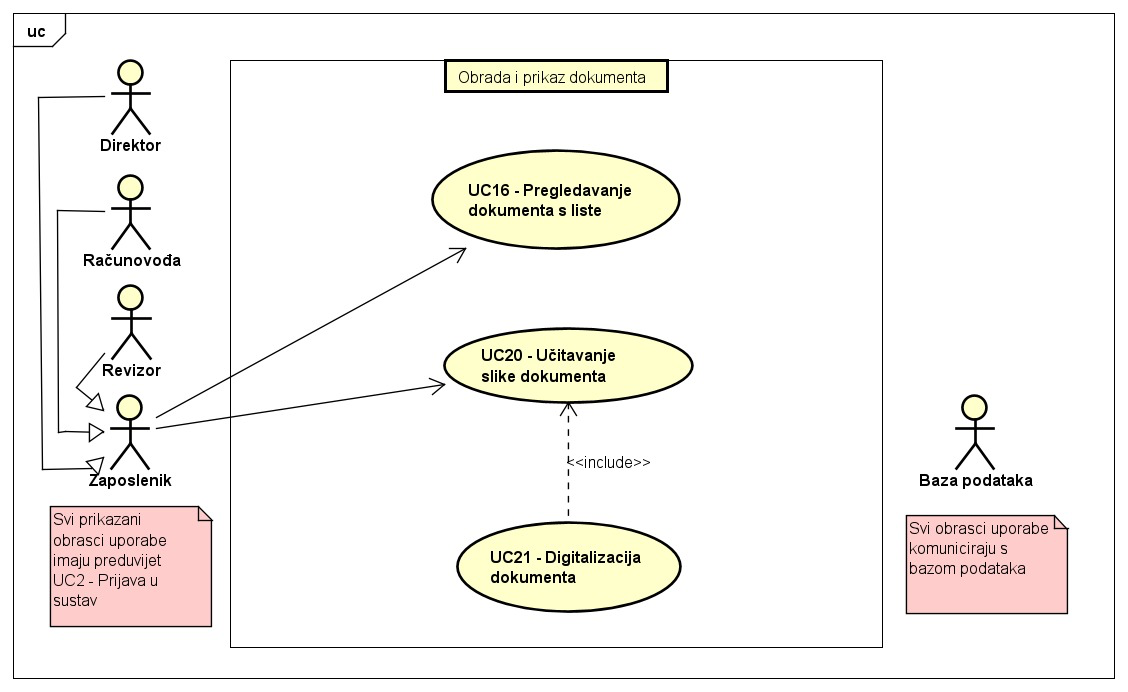
\includegraphics[width=\textwidth]{slike/3.1.1 dijagrami/ObradaIPrikazDokumenata.PNG}
						\caption{Dijagram obrasca uporabe, funkcionalnost svih aktora}
						\label{Obrazac1} 
					\end{figure}
					
					\begin{figure}[H]
						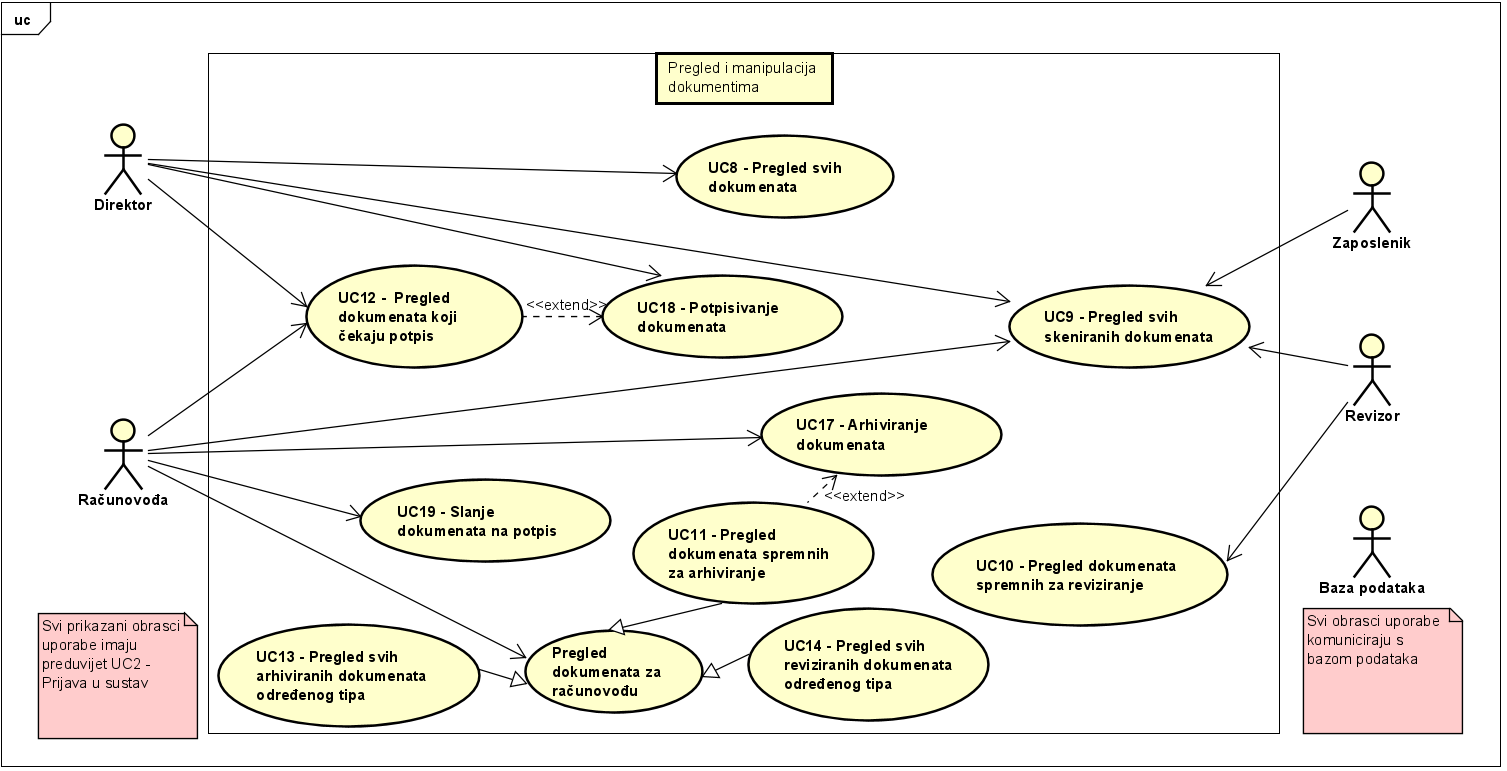
\includegraphics[width=\textwidth]{slike/3.1.1 dijagrami/PregledIManipulacijaDokumentima_v2.PNG}
						\caption{Dijagram obrasca uporabe, funkcionalnost svih aktora}
						\label{Obrazac2} 
					\end{figure}
					
					\begin{figure}[H]
						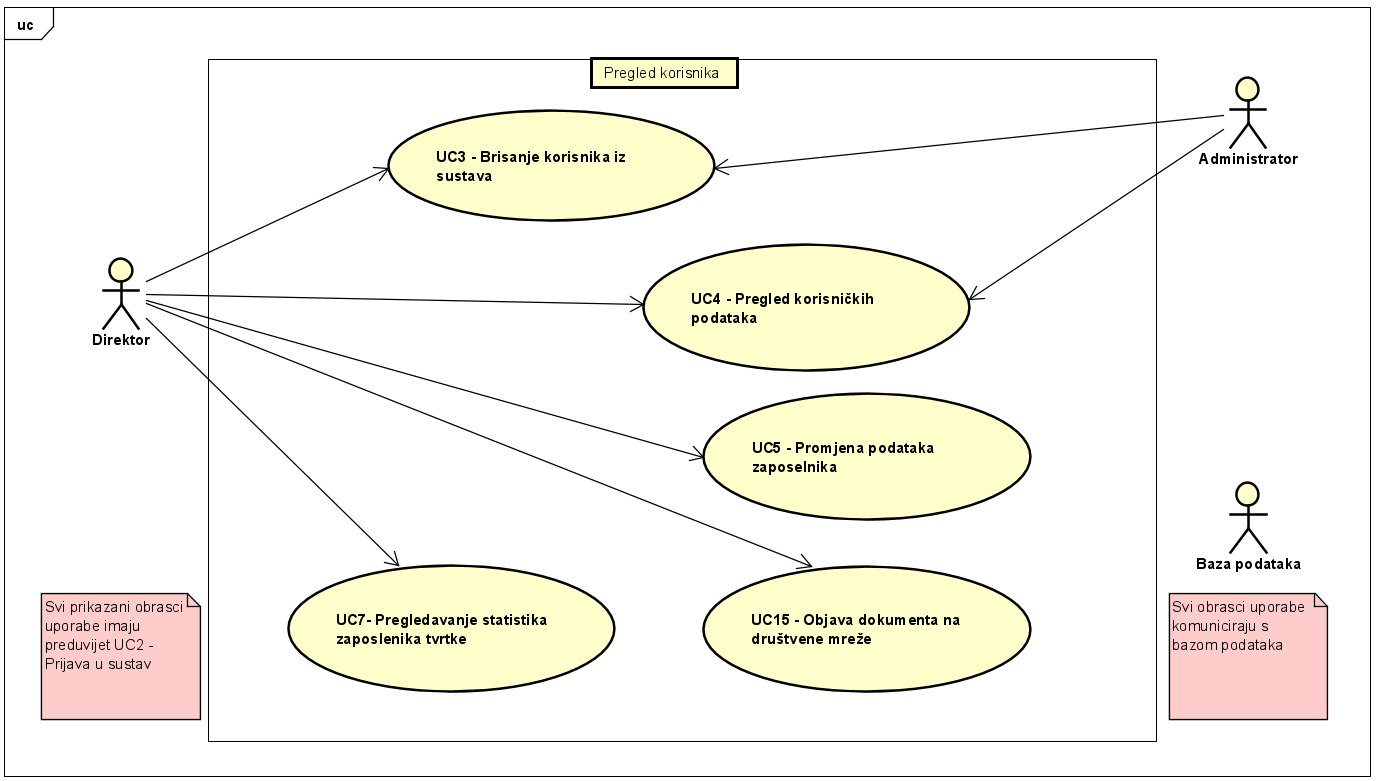
\includegraphics[width=\textwidth]{slike/3.1.1 dijagrami/PregledKorisnika.PNG}
						\caption{Dijagram obrasca uporabe, funkcionalnost Direktora i Administratora}
						\label{Obrazac3} 
					\end{figure}
					
					\begin{figure}[H]
						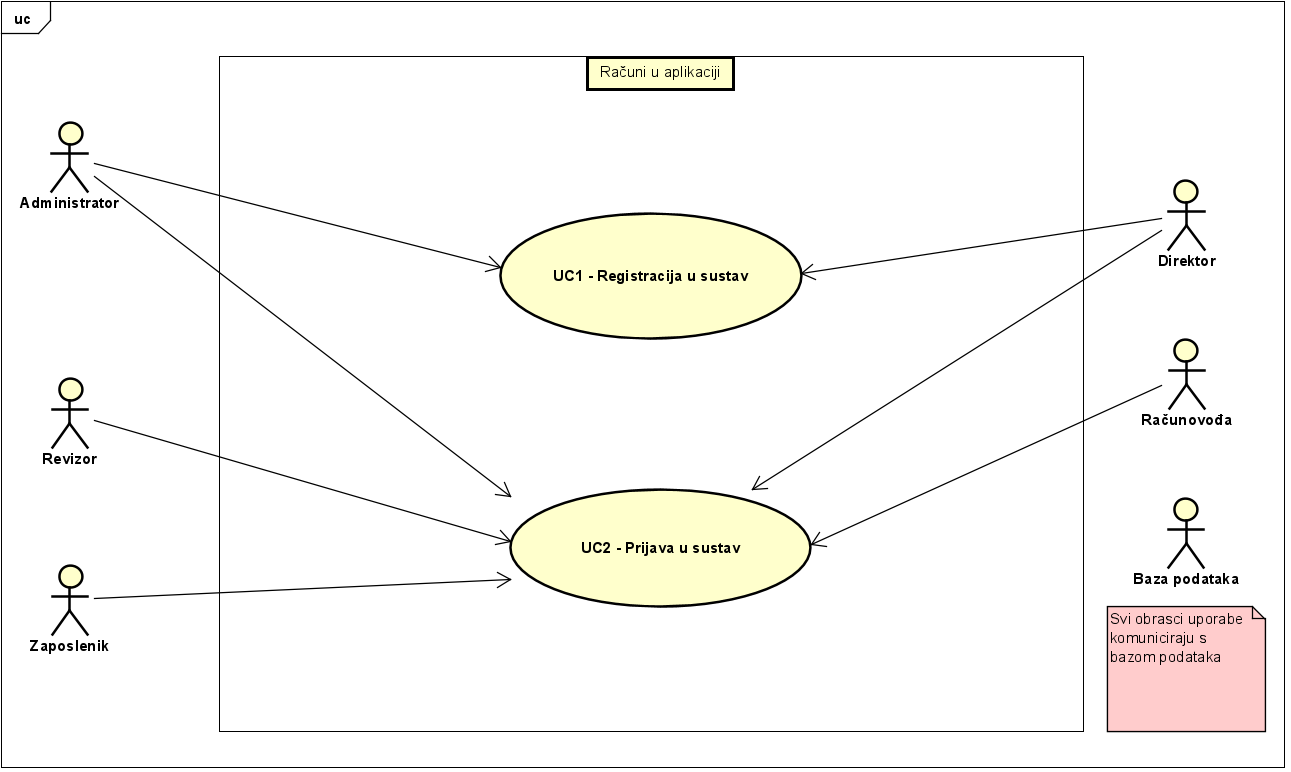
\includegraphics[width=\textwidth]{slike/3.1.1 dijagrami/RačuniUAplikaciji.PNG}
						\caption{Dijagram obrasca uporabe, funkcionalnost svih aktora}
						\label{Obrazac4} 
					\end{figure}
					
				\eject		
				
			\subsection{Sekvencijski dijagrami}
				
				\textbf{Obrazac uporabe UC2 - Prijava u sustav}\
				
				Korisnik unosi svoje osobne podatke. Sustav provjerava u bazi podataka jesu li uneseni podaci ispravni. Ako jesu, korisnik se prijavi u sustav. No ako uneseni podaci ne odgovaraju niti jednom registriranom korisniku u bazi, sustav korisniku šalje obavijest da su osobni podaci neispravni i daje mu priliku za ponovnu prijavu.
				\begin{figure}[H]
					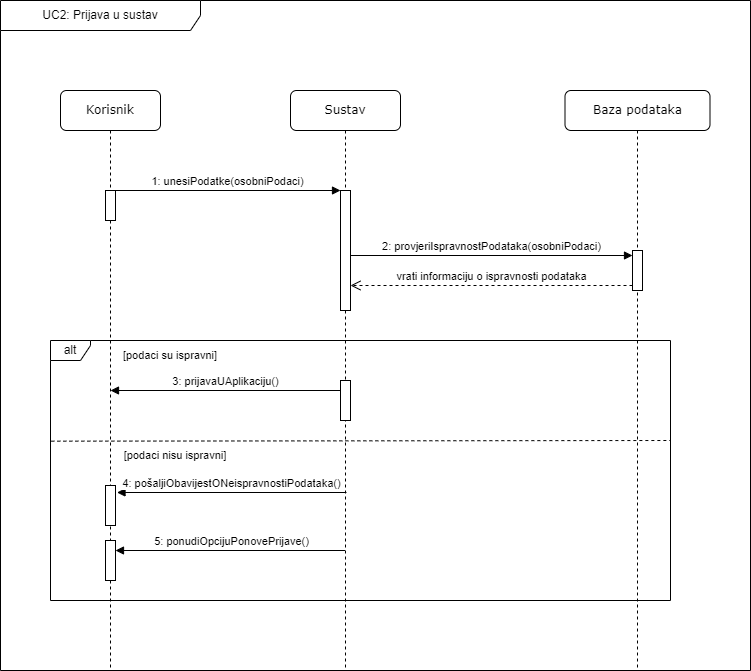
\includegraphics[width=\textwidth]{slike/sekvencijski_dijagram_UC2.PNG} %veličina u odnosu na širinu linije
					\caption{Slika broj: Sekvencijski dijagram za UC2}
					\label{fig:UC2} %label mora biti drugaciji za svaku sliku
				\end{figure}
				\clearpage

				\textbf{Obrazac uporabe UC9 - Pregled skeniranih dokumenata}\
				
				Korisnik odabire pregled popisa svih dokumenata koje je skenirao. Sustav pretraži u bazi njegove skenirane dokumente i vraća ih korisniku na uvid.
				\begin{figure}[H]
					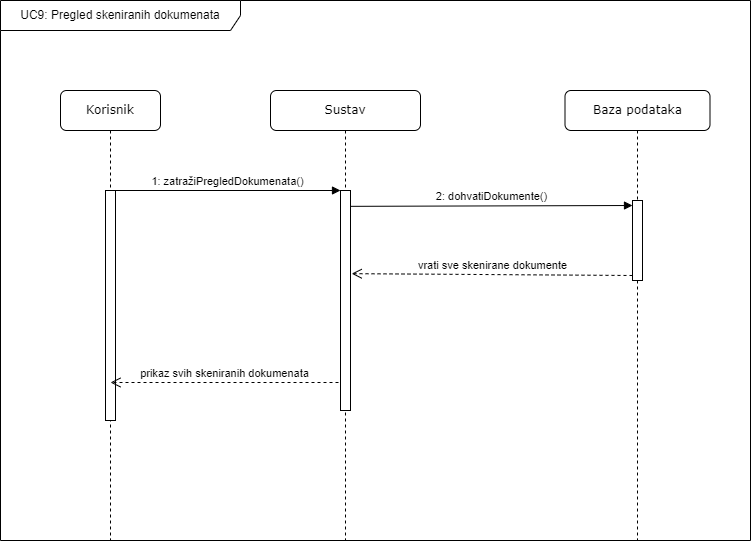
\includegraphics[width=\textwidth]{slike/sekvencijski_dijagram_UC9.PNG} %veličina u odnosu na širinu linije
					\caption{Slika broj: Sekvencijski dijagram za UC9}
					\label{fig:UC9} %label mora biti drugaciji za svaku sliku
				\end{figure}
				\clearpage

				\textbf{Obrazac uporabe UC21 - Digitalizacija dokumenta}\
				
				Korisnik šalje sliku  u sustav koji zatim tu sliiku učitava i pregledava je li na slici dokument. Ako je, onda na njega primjenjuje OCR te novonastali dokument sprema u bazu podataka. Ako na slici nije očitan dokument, sustav korisniku šalje obavijst da učitana slika ne sadrži dokument te mu daje opciju da priloži novu sliku.
				\begin{figure}[H]
					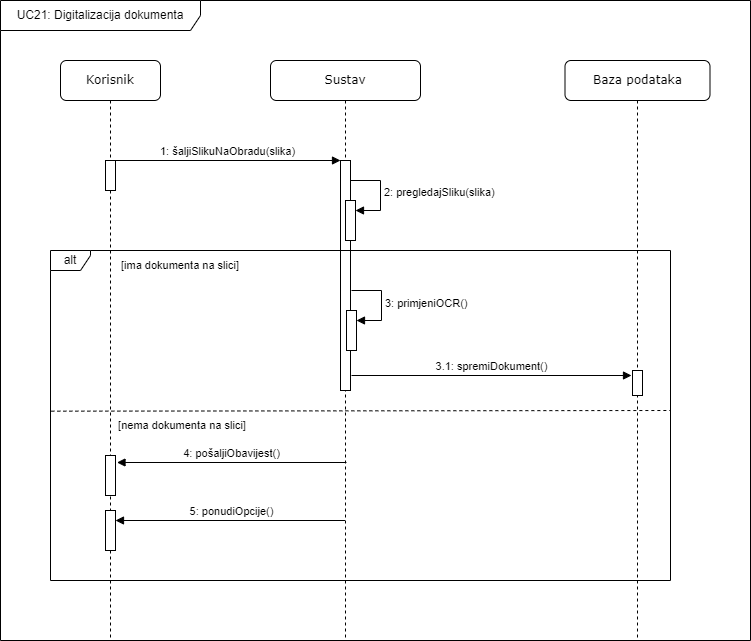
\includegraphics[width=\textwidth]{slike/sekvencijski_dijagram_UC21.PNG} %veličina u odnosu na širinu linije
					\caption{Slika broj: Sekvencijski dijagram za UC21}
					\label{fig:UC21} %label mora biti drugaciji za svaku sliku
				\end{figure}		
				\clearpage

				\eject
	
		\section{Ostali zahtjevi}

			 	\begin{packed_item}
			 	
			 	\item Sustav treba omogućiti rad više korisnika u istom razdoblju
			 	\item Korisničko sučelje ne smije imati greške(bug-ove) kojima je moguće da klijent ima pristup ovlastima koje mu ne bi trebale biti dozvoljene
			 	\item Sustav treba biti implementiran kao mobilna aplikacija koja koristeći objektno-orijentirane jezike
			 	\item Korisničko sučelje treba biti u stanju podržavati različite dijakritičke znakove u tekstualnom sučelju
			 	\item Dohvaćanje podataka iz baze podataka i njihov prikaz ne smije trajati duže od nekoliko sekundi
			 	\item Veza s bazom mora biti sigurna i zaštićena kako bi bila otporna na krađu klasificiranih podataka tvrtke
			 	\item Sustav treba imati intuitivno i jednostavno korisničko sučelje za koje nisu potrebne upute korištenja
			 	\item Eventualna nadogradnja sustava ne smije brisati značajke aplikacije protiv volje korisnika aplikacije
			 		
			 	\end{packed_item}
			 
			 
			 
	
	\chapter{Arhitektura i dizajn sustava}
		
		%\textbf{\textit{dio 1. revizije}}\\

		%\textit{ Potrebno je opisati stil arhitekture te identificirati: podsustave, preslikavanje na radnu platformu, spremišta podataka, mrežne protokole, globalni upravljački tok i sklopovsko-programske zahtjeve. Po točkama razraditi i popratiti odgovarajućim skicama:}
%	\begin{itemize}
%		\item 	\textit{izbor arhitekture temeljem principa oblikovanja pokazanih na predavanjima (objasniti zašto ste baš odabrali takvu arhitekturu)}
%		\item 	\textit{organizaciju sustava s najviše razine apstrakcije (npr. klijent-poslužitelj, baza podataka, datotečni sustav, grafičko sučelje)}
%		\item 	\textit{organizaciju aplikacije (npr. slojevi frontend i backend, MVC arhitektura) }		
%	\end{itemize}
	
		{Arhitektura rješenja se sastoji od 3 sustava: Mobilne aplikacije(Frontend), Web aplikacije(Backend) i Baze podataka.}
		
		{\underbar{Mobilna aplikacija} je softver namjenjen pokretanju na mobilnim uređajima poput mobitela i tableta. Ona pomoću API-a \textbf{(Application programming interface)} komunicira s web aplikacijom koja se brine za logiku. API je je skup pravila, protokola i definicija koje omogućuje komunikaciju između različitih programa ili aplikacija. Sama komunikacija se odvija pomoću HTTPS-a \textbf{(Hypertext Transfer Protocol Secure)}, što je sigurnija inačica HTTP-a \textbf{(Hypertext Transfer Protocol)} koji omogućuje kkomunikaciju na internetu. Kada web aplikacija primi zahtjev od mobilne aplikacije, ona ovisno o zahtjevu, pristupa bazi podataka kako bi dohvatila, promjenila ili dodala informacije. Ovisno o zahtjevu, web aplikacija vraća odgovor na orginalni zahtjev mobilne aplikacije i mobilna aplikacija prikazuje dobivene informacije kroz svoje sučelje.}
		
		{Mobilna aplikacija je razvijena pomoću programskog jezika \textit{Dart} te radnog okvira \textit{Flutter} unutar razvojnog okruženja \textit{Android Studio}. Web aplikacija je razvijena pomoću programskog jezika \textit{Python} te radnog okvira \textit{FastAPI} unutar razvojnog okruženja \textit{PyCharm} te je postavljena na \textit{render.com}. Sve podatke pohranjujemo unutar \textit{PostgreSQL} baze podataka koja je na \textit{Azure}-u.}
		
		{Aplikacija se temelji na MVC konceptu u modernijoj izvedbi koja je na web aplikaciji bliža tipičnoj arhitekturi fastapi aplikacija:}
		\begin{itemize}
			\item {\textbf{Model} - Model predstavlja strukture podatakae. On pristupa bazi podataka, te upravlja podacima. Unutar našeg rješenja, postoji poseban sloj u web aplikaciji koji komunicira s bazom podataka (CRUD klase).}
			\item {\textbf{View} - Pogled predstavlja korisničko sučelje aplikacije te prikazuje sve informacije korisniku. Pomoću njega, korisnik može imati interakciju s ostatkom aplikacije. U našoj arhitekturi, to bi bila mobilna aplikacija koja prikazuje sve informacije i sama po sebi ima minimalnu logiku te primarna svrha je prikaz informacija korisniku.}
			\item {\textbf{Controller} - Kontroler postoji između Viewa i Modela te služi da bi primao zahtjeve od Viewa, slao odgovore natrag Viewu, vrši poslovnu logiku te proslijeduje zahtjeve pripadnom djelu modela. Unutar naše izvedbe, Controller je dio Web aplikacije koji prima zahtjeve od mobilne aplikacije, vrši poslovnu logiku nad njima te prosljeđuje potrebne podatke iz zahtjeva modelu te od modela dobiva natrag podatke koje u prikladnom obliku prosljeđuje mobilnoj aplikaciji. U našoj izvedbi je izveden pomoću route funckija i Service klasa.}
		\end{itemize} 
		
				

	
				
		\section{Baza podataka}
			
			%\textbf{\textit{dio 1. revizije}}\\
			
			{Koristimo relacijsku bazu podataka s implementacijom pomoću PostgreSQL-a. Za opis naše baze podataka koristimo DBML.  DBML (Database Markup Language) je jezik označavanja koji omogućuje deklarativno opisivanje relacijskih baza podataka.  Time možemo jednostavno definirati strukture baze podataka pomoću tekstualnog zapisa.  Zadaća baze podataka je da olakša i ubrza pristup podacima za daljnju obradu ili pronalaženje arhiviranih podataka. Glavne komponente naše baze podataka su:}
				\begin{packed_item}
					\item 	\textbf{documents}
					\item 	\textbf{users}
					\item 	\textbf{signatures}
					\item 	\textbf{audits}
					\item 	\textbf{archive}
					\item 	\textbf{image}
					\item 	\textbf{user\textunderscore role}
					\item	\textbf{roles}
				\end{packed_item}
		
			\subsection{Opis tablica}
			
				
				\textbf{Documents} 
				{  Sadrži informacije o dokumentima, uključujući vrstu dokumenta, sliku dokumenta, sažetak, status, vlasnika i vremensku oznaku skeniranja. Ovaj entitet u vezi je \textit{One-to-Many} s entitetom \textbf{users} preko atributa \textit{owner\_id}, u vezi je \textit{One-to-Many} s entitetom \textbf{signatures} preko atributa \textit{id}, u vezi je \textit{One-to-Many} s entitetom \textbf{audits} preko atributa \textit{id}, u vezi je \textit{One-to-Many} s entitetom \textbf{archive} preko atributa \textit{id}, u vezi je \textit{One-to-One} s entitetom \textbf{image} preko atributa \textit{image\_id}, u vezi je \textit{Many-to-One} s entitetom \textbf{users} preko atributa \textit{owner\_id}.}
				
				
				\begin{longtblr}[
					label=none,
					entry=none
					]{
						width = \textwidth,
						colspec={|X[8,l]|X[5, l]|X[20, l]|}, 
						rowhead = 1,
					} 
					\hline \SetCell[c=3]{c}{\textbf{documents}}	 \\ \hline[3pt]
					\SetCell{LightGreen}id & INT & identifikacijski broj dokumenta  	\\ \hline
					document\_type	& ENUM & tip skeniranog dokumenta: račun, ponuda ili interni	\\ \hline 
					\SetCell{LightBlue}image\_id & INT & identifikacijski broj slike dokumenta  \\ \hline 
					summary & TEXT	& tekst koji sadrži skenirani dokument 		\\ \hline 
					document\_status	& ENUM & trenutni status dokumenta: skeniran, odobren, odbijen, potpisan, reviziran, potpisan i arhiviran ili arhiviran 	\\ \hline 
					\SetCell{LightBlue}owner\_id & INT & identifikacijski broj korisnika koji je skenirao dokument \\ \hline
					scan\_timestamp & DATETIME & oznaka datuma i vremena skeniranja dokumenta \\ \hline
				\end{longtblr}
				
				\textbf{Users} 
				{  Sprema informacije o korisnicima, uključujući korisničko ime i lozinku, ime i prezime korisnika te email. Ovaj entitet u vezi je \textit{One-to-Many} s entitetom \textbf{documents} preko atributa \textit{id}, u vezi je \textit{One-to-Many} s entitetom \textbf{signatures} preko atributa \textit{id}, u vezi je \textit{One-to-Many} s entitetom \textbf{audits} preko atributa \textit{id}, u vezi je \textit{One-to-Many} s entitetom \textbf{archive} preko atributa \textit{id}, u vezi je \textit{One-to-Many} s entitetom \textbf{user\textunderscore role} preko atributa \textit{id}.}
				
				\begin{longtblr}[
					label=none,
					entry=none
					]{
						width = \textwidth,
						colspec={|X[8,l]|X[5, l]|X[20, l]|}, 
						rowhead = 1,
					} 
					\hline \SetCell[c=3]{c}{\textbf{users}}	 \\ \hline[3pt]
					\SetCell{LightGreen}id & INT & identifikacijski broj korisnika  	\\ \hline
					email & VARCHAR & email korisnika \\ \hline
					first\_name & VARCHAR & ime korisnika \\ \hline
					last\_name & VARCHAR & prezime korisnika \\ \hline
					username	& VARCHAR & korisničko ime za prijavu korisnika	\\ \hline 
					password & VARCHAR & šifa za prijavu korisnika  \\ \hline 
				\end{longtblr}
				
				
				\textbf{Signatures}
				{  Služi za praćenje potpisa na dokumentima, s informacijama o korisniku koji je potpisao, statusu potpisa i vremenskoj oznaci potpisa. Ovaj entitet u vezi je \textit{Many-to-One} s entitetom \textbf{users} preko atributa \textit{sign\_by}, u vezi je \textit{One-to-One} s entitetom \textbf{documents} preko atributa \textit{document\_id}.}
				
				\begin{longtblr}[
					label=none,
					entry=none
					]{
						width = \textwidth,
						colspec={|X[8,l]|X[5, l]|X[20, l]|}, 
						rowhead = 1,
					} 
					\hline \SetCell[c=3]{c}{\textbf{signatures}}	 \\ \hline[3pt]
					\SetCell{LightGreen}signature\_id & INT & identifikacijski broj potpisanog dokumenta  	\\ \hline
					\SetCell{LightBlue}document\_id	& INT & identifikacijski broj dokumenta	\\ \hline 
					\SetCell{LightBlue}sign\_by & INT & identifikacijski broj korisnika koji je potpisao ili treba potpisati dokument  \\ \hline 
					status & ENUM & status dokumenta za potpisivanje: potpisan ili čeka na potpisivanje \\ \hline
					signed\_at & DATETIME & oznaka datuma i vremena potpisivanja dokumenta \\ \hline
				\end{longtblr}
				
				\textbf{Audits}
				{  Sadrži podatke o revizijama dokumenata, uključujući korisnika koji je obavio reviziju, status revizije i vremensku oznaku. Ovaj entitet u vezi je \textit{Many-to-One} s entitetom \textbf{users} preko atributa \textit{audited\_by}, u vezi je \textit{One-to-One} s entitetom \textbf{documents} preko atributa \textit{document\_id}.}
				
				\begin{longtblr}[
					label=none,
					entry=none
					]{
						width = \textwidth,
						colspec={|X[8,l]|X[5, l]|X[20, l]|}, 
						rowhead = 1,
					} 
					\hline \SetCell[c=3]{c}{\textbf{audits}}	 \\ \hline[3pt]
					\SetCell{LightGreen}audit\_id & INT & identifikacijski broj reviziranog dokumenta  	\\ \hline
					\SetCell{LightBlue}document\_id	& INT & identifikacijski broj dokumenta	\\ \hline 
					\SetCell{LightBlue}audited\_by & INT & identifikacijski broj korisnika koji je revizirao ili treba revizirati dokument  \\ \hline 
					status & ENUM & status dokumenta za reviziju: reviziran ili čeka na reviziranje \\ \hline
					audited\_at & DATETIME & oznaka datuma i vremena reviziranja dokumenta \\ \hline
				\end{longtblr}
				
				\textbf{Archive}
				{  Koristi se za praćenje arhiviranja dokumenata, s informacijama o korisniku koji je arhivirao dokument, statusu arhiviranja, vremenskoj oznaci i broju arhive. Ovaj entitet u vezi je \textit{One-to-One} s entitetom \textbf{documents} preko atributa \textit{document\_id}, u vezi je \textit{Many-to-One} s entitetom \textbf{users} preko atributa \textit{archive\_by}.}
				
				\begin{longtblr}[
					label=none,
					entry=none
					]{
						width = \textwidth,
						colspec={|X[8,l]|X[5, l]|X[20, l]|}, 
						rowhead = 1,
					} 
					\hline \SetCell[c=3]{c}{\textbf{archive}}	 \\ \hline[3pt]
					\SetCell{LightGreen}archive\_number & INT & identifikacijski broj arhiviranog dokumenta  	\\ \hline
					\SetCell{LightBlue}document\_id	& INT & identifikacijski broj dokumenta	\\ \hline 
					\SetCell{LightBlue}archive\_by & INT & identifikacijski broj korisnika koji je arhivirao ili treba arhivirati dokument  \\ \hline 
					status & ENUM & status dokumenta za arhiviranje: arhiviran ili čeka na arhiviranje \\ \hline
					archived\_at & DATETIME & oznaka datuma i vremena arhiviranja dokumenta \\ \hline
				\end{longtblr}
				
				\textbf{Image}
				{  Sprema slike dokumenata. Ovaj entitet u vezi je \textit{One-to-One} s entitetom \textbf{documents} preko atributa \textit{id}.}
				
				\begin{longtblr}[
					label=none,
					entry=none
					]{
						width = \textwidth,
						colspec={|X[8,l]|X[5, l]|X[20, l]|}, 
						rowhead = 1,
					} 
					\hline \SetCell[c=3]{c}{\textbf{image}}	 \\ \hline[3pt]
					\SetCell{LightGreen}id & INT & identifikacijski broj slike dokumenta  	\\ \hline
					image & VARCHAR & putanja do spremljene slike \\ \hline
				\end{longtblr}
				
				\textbf{Roles}
				{  Definira različite uloge korisnika u sistemu. Ovaj entitet u vezi je \textit{One-to-Many} s entitetom \textbf{user\textunderscore role} preko atributa \textit{role\_id}.}
				
				
				\begin{longtblr}[
					label=none,
					entry=none
					]{
						width = \textwidth,
						colspec={|X[8,l]|X[5, l]|X[20, l]|}, 
						rowhead = 1,
					} 
					\hline \SetCell[c=3]{c}{\textbf{roles}}	 \\ \hline[3pt]
					\SetCell{LightGreen}role\_id & INT & identifikacijski broj kategorije korisnika  	\\ \hline
					role\_name & VARCHAR & ime uloge korisnika \\ \hline
				\end{longtblr}
				
				\textbf{User\textunderscore role}
				{  Tablica koja povezuje korisnike s njihovim ulogama. Ovaj entitet u vezi je \textit{Many-to-One} s entitetom \textbf{roles} preko atributa \textit{role\_id}, u vezi je \textit{Many-to-One} s entitetom \textbf{users} preko atributa \textit{user\_id}.}
				
				\begin{longtblr}[
					label=none,
					entry=none
					]{
						width = \textwidth,
						colspec={|X[8,l]|X[5, l]|X[20, l]|}, 
						rowhead = 1,
					} 
					\hline \SetCell[c=3]{c}{\textbf{user\textunderscore role}}	 \\ \hline[3pt]
					\SetCell{LightGreen}user\_id & INT & identifikacijski broj korisnika  	\\ \hline
					\SetCell{LightGreen}role\_id & INT & identifikacijski broj kategorije korisnika \\ \hline
				\end{longtblr}
				
				
			
			\subsection{Dijagram baze podataka}
				
				\begin{figure}[H]
					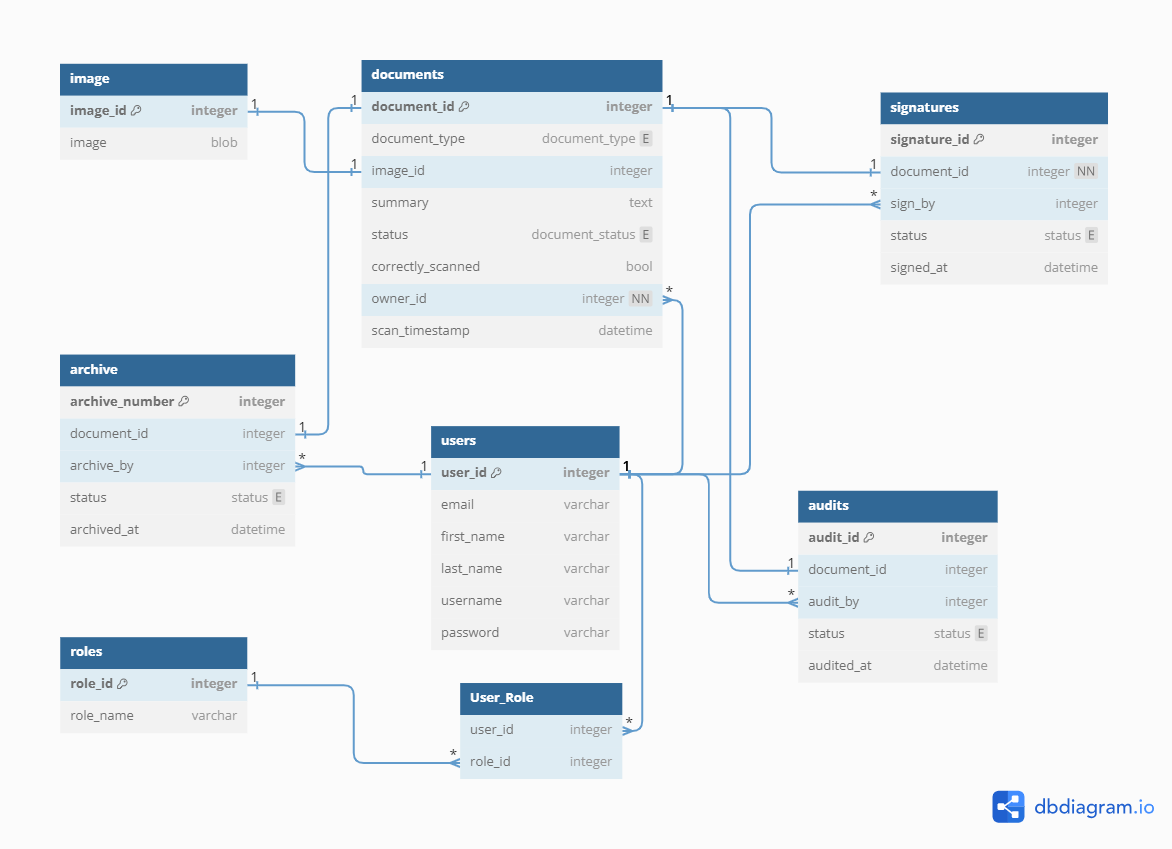
\includegraphics[width=\textwidth]{slike/dijagramBaze.PNG} 
					\caption{Dijagram baze podataka}
					\label{fig:dijagramBaze}
				\end{figure}
			
			\eject
			
			
		\section{Dijagram razreda}
		
			%\textit{Potrebno je priložiti dijagram razreda s pripadajućim opisom. Zbog preglednosti je moguće dijagram razlomiti na više njih, ali moraju biti grupirani prema sličnim razinama apstrakcije i srodnim funkcionalnostima.}\\
			
			%\textbf{\textit{dio 1. revizije}}\\
			
			%\textit{Prilikom prve predaje projekta, potrebno je priložiti potpuno razrađen dijagram razreda vezan uz \textbf{generičku funkcionalnost} sustava. Ostale funkcionalnosti trebaju biti idejno razrađene u dijagramu sa sljedećim komponentama: nazivi razreda, nazivi metoda i vrste pristupa metodama (npr. javni, zaštićeni), nazivi atributa razreda, veze i odnosi između razreda.}\\
			
			\begin{figure}[H]
				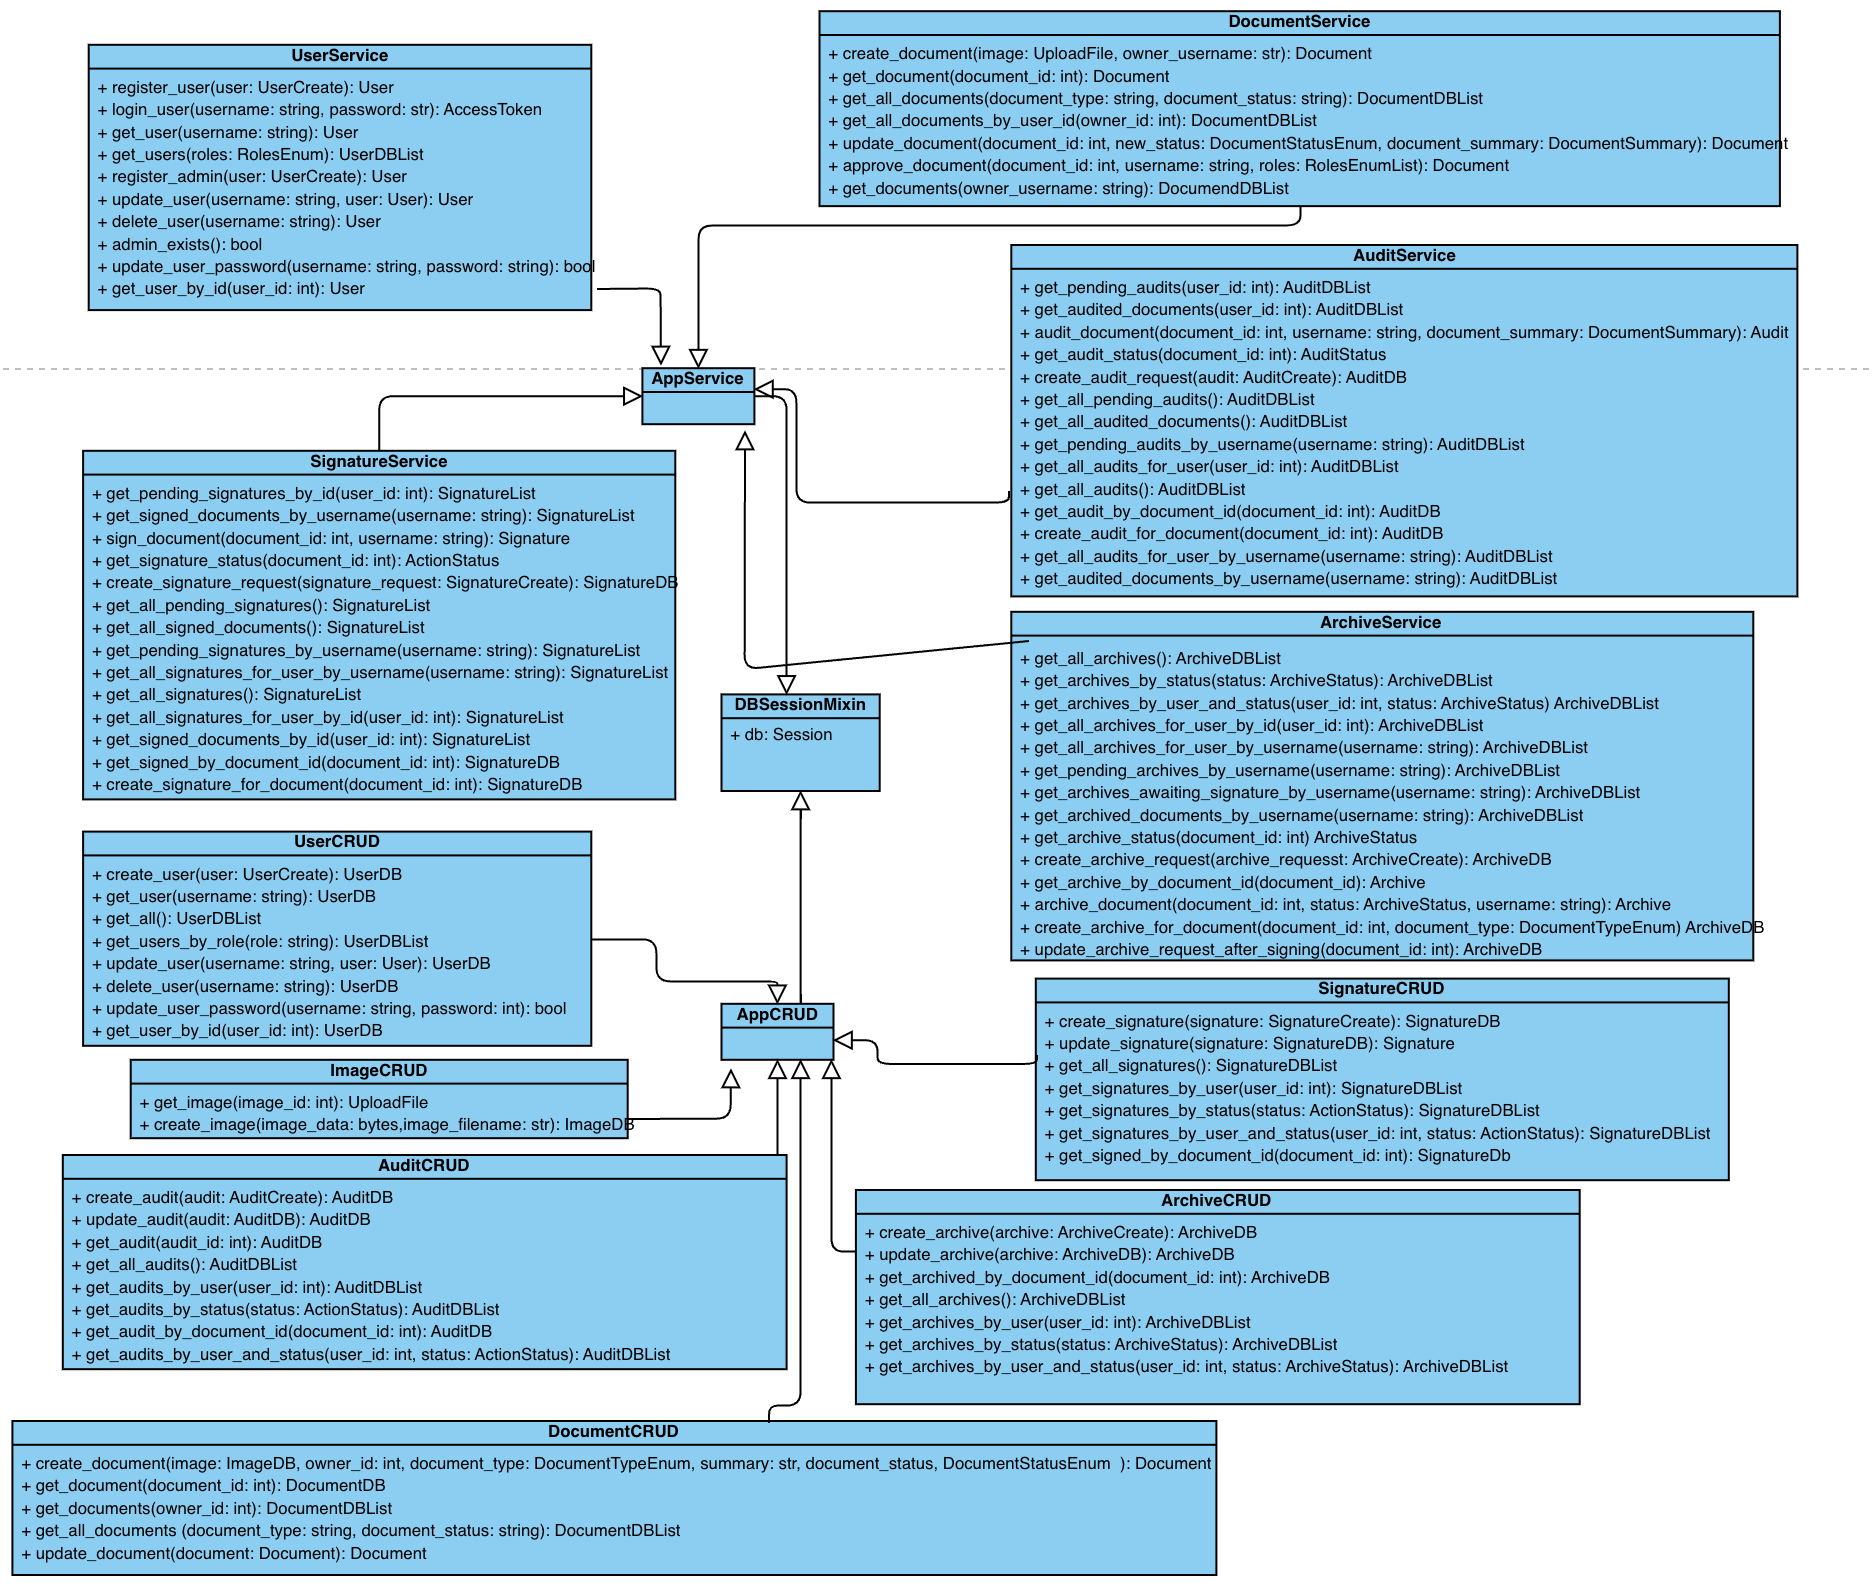
\includegraphics[width=\textwidth]{slike/razredi_serviceCRUD.png} 
				\caption{Dijagram razreda - servisi i CRUD}
				\label{fig:dijagramRazreda1}
			\end{figure}
			
			\begin{figure}[H]
				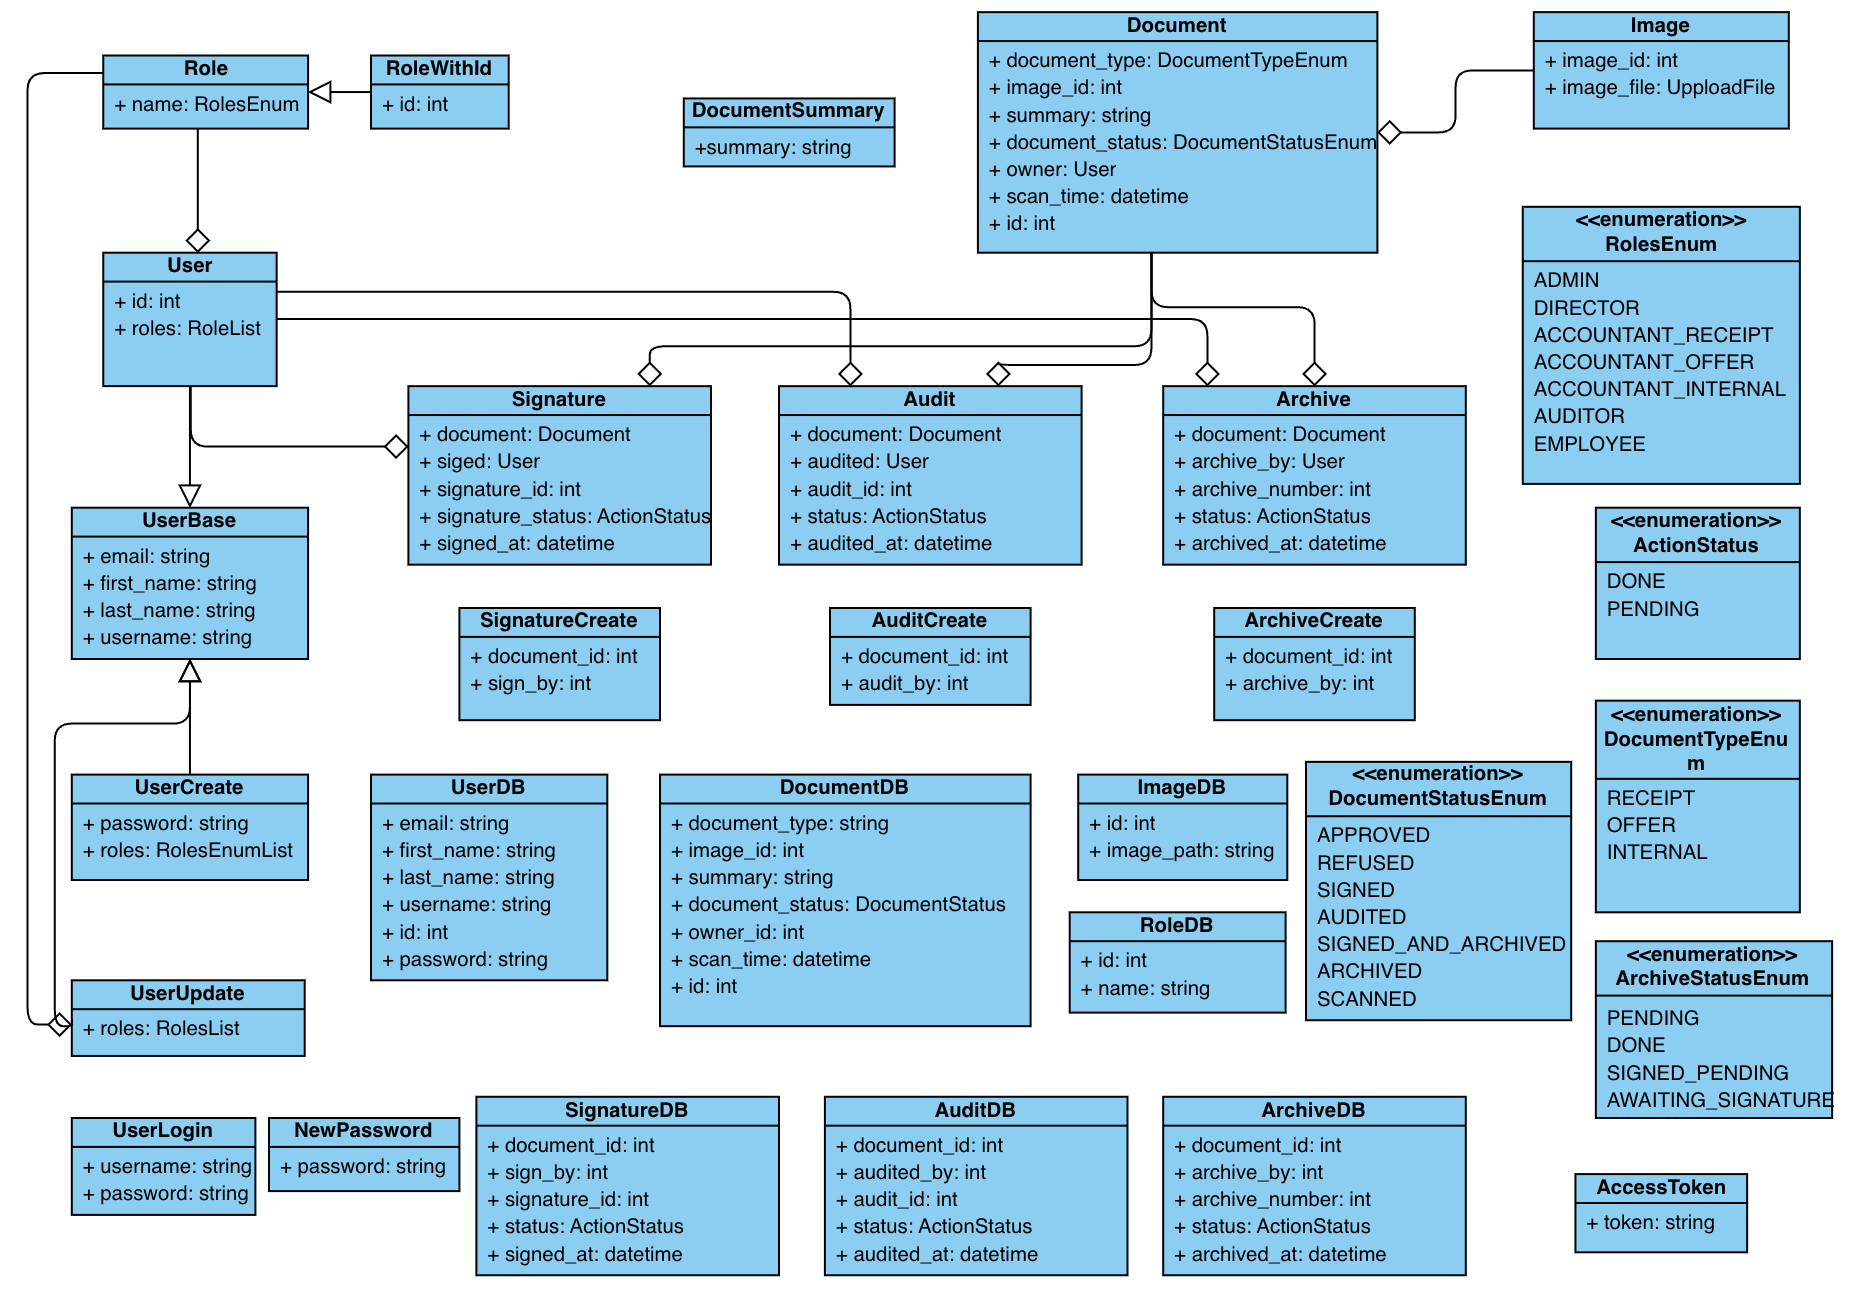
\includegraphics[width=\textwidth]{slike/razredi_shemaModel.png} 
				\caption{Dijagram razreda - shema i model}
				\label{fig:dijagramRazreda2}
			\end{figure}
			
			%\textbf{\textit{dio 2. revizije}}\\			
			
			%\textit{Prilikom druge predaje projekta dijagram razreda i opisi moraju odgovarati stvarnom stanju implementacije}
			
			
			
			\eject
		
		\section{Dijagram stanja}
			
			
			%\textbf{\textit{dio 2. revizije}}\\
			
			%\textit{Potrebno je priložiti dijagram stanja i opisati ga. Dovoljan je jedan dijagram stanja koji prikazuje \textbf{značajan dio funkcionalnosti} sustava. Na primjer, stanja korisničkog sučelja i tijek korištenja neke ključne funkcionalnosti jesu značajan dio sustava, a registracija i prijava nisu. }
			
			
			\eject 
		
		\section{Dijagram aktivnosti}
			
			%\textbf{\textit{dio 2. revizije}}\\
			
			 %\textit{Potrebno je priložiti dijagram aktivnosti s pripadajućim opisom. Dijagram aktivnosti treba prikazivati značajan dio sustava.}

			{Na dijagramu aktivnosti prikazan je proces digitalizacije dokumenta. Nakon prijave zaposlenika slijedi odabir slike dokumenta koji se šalje na obradu. Stvara se objekt dokumenta koji se zatim redom šalje na reviziju, arhiviranje i po potrebi na potpis.}

			 \begin{figure}[H]
			 	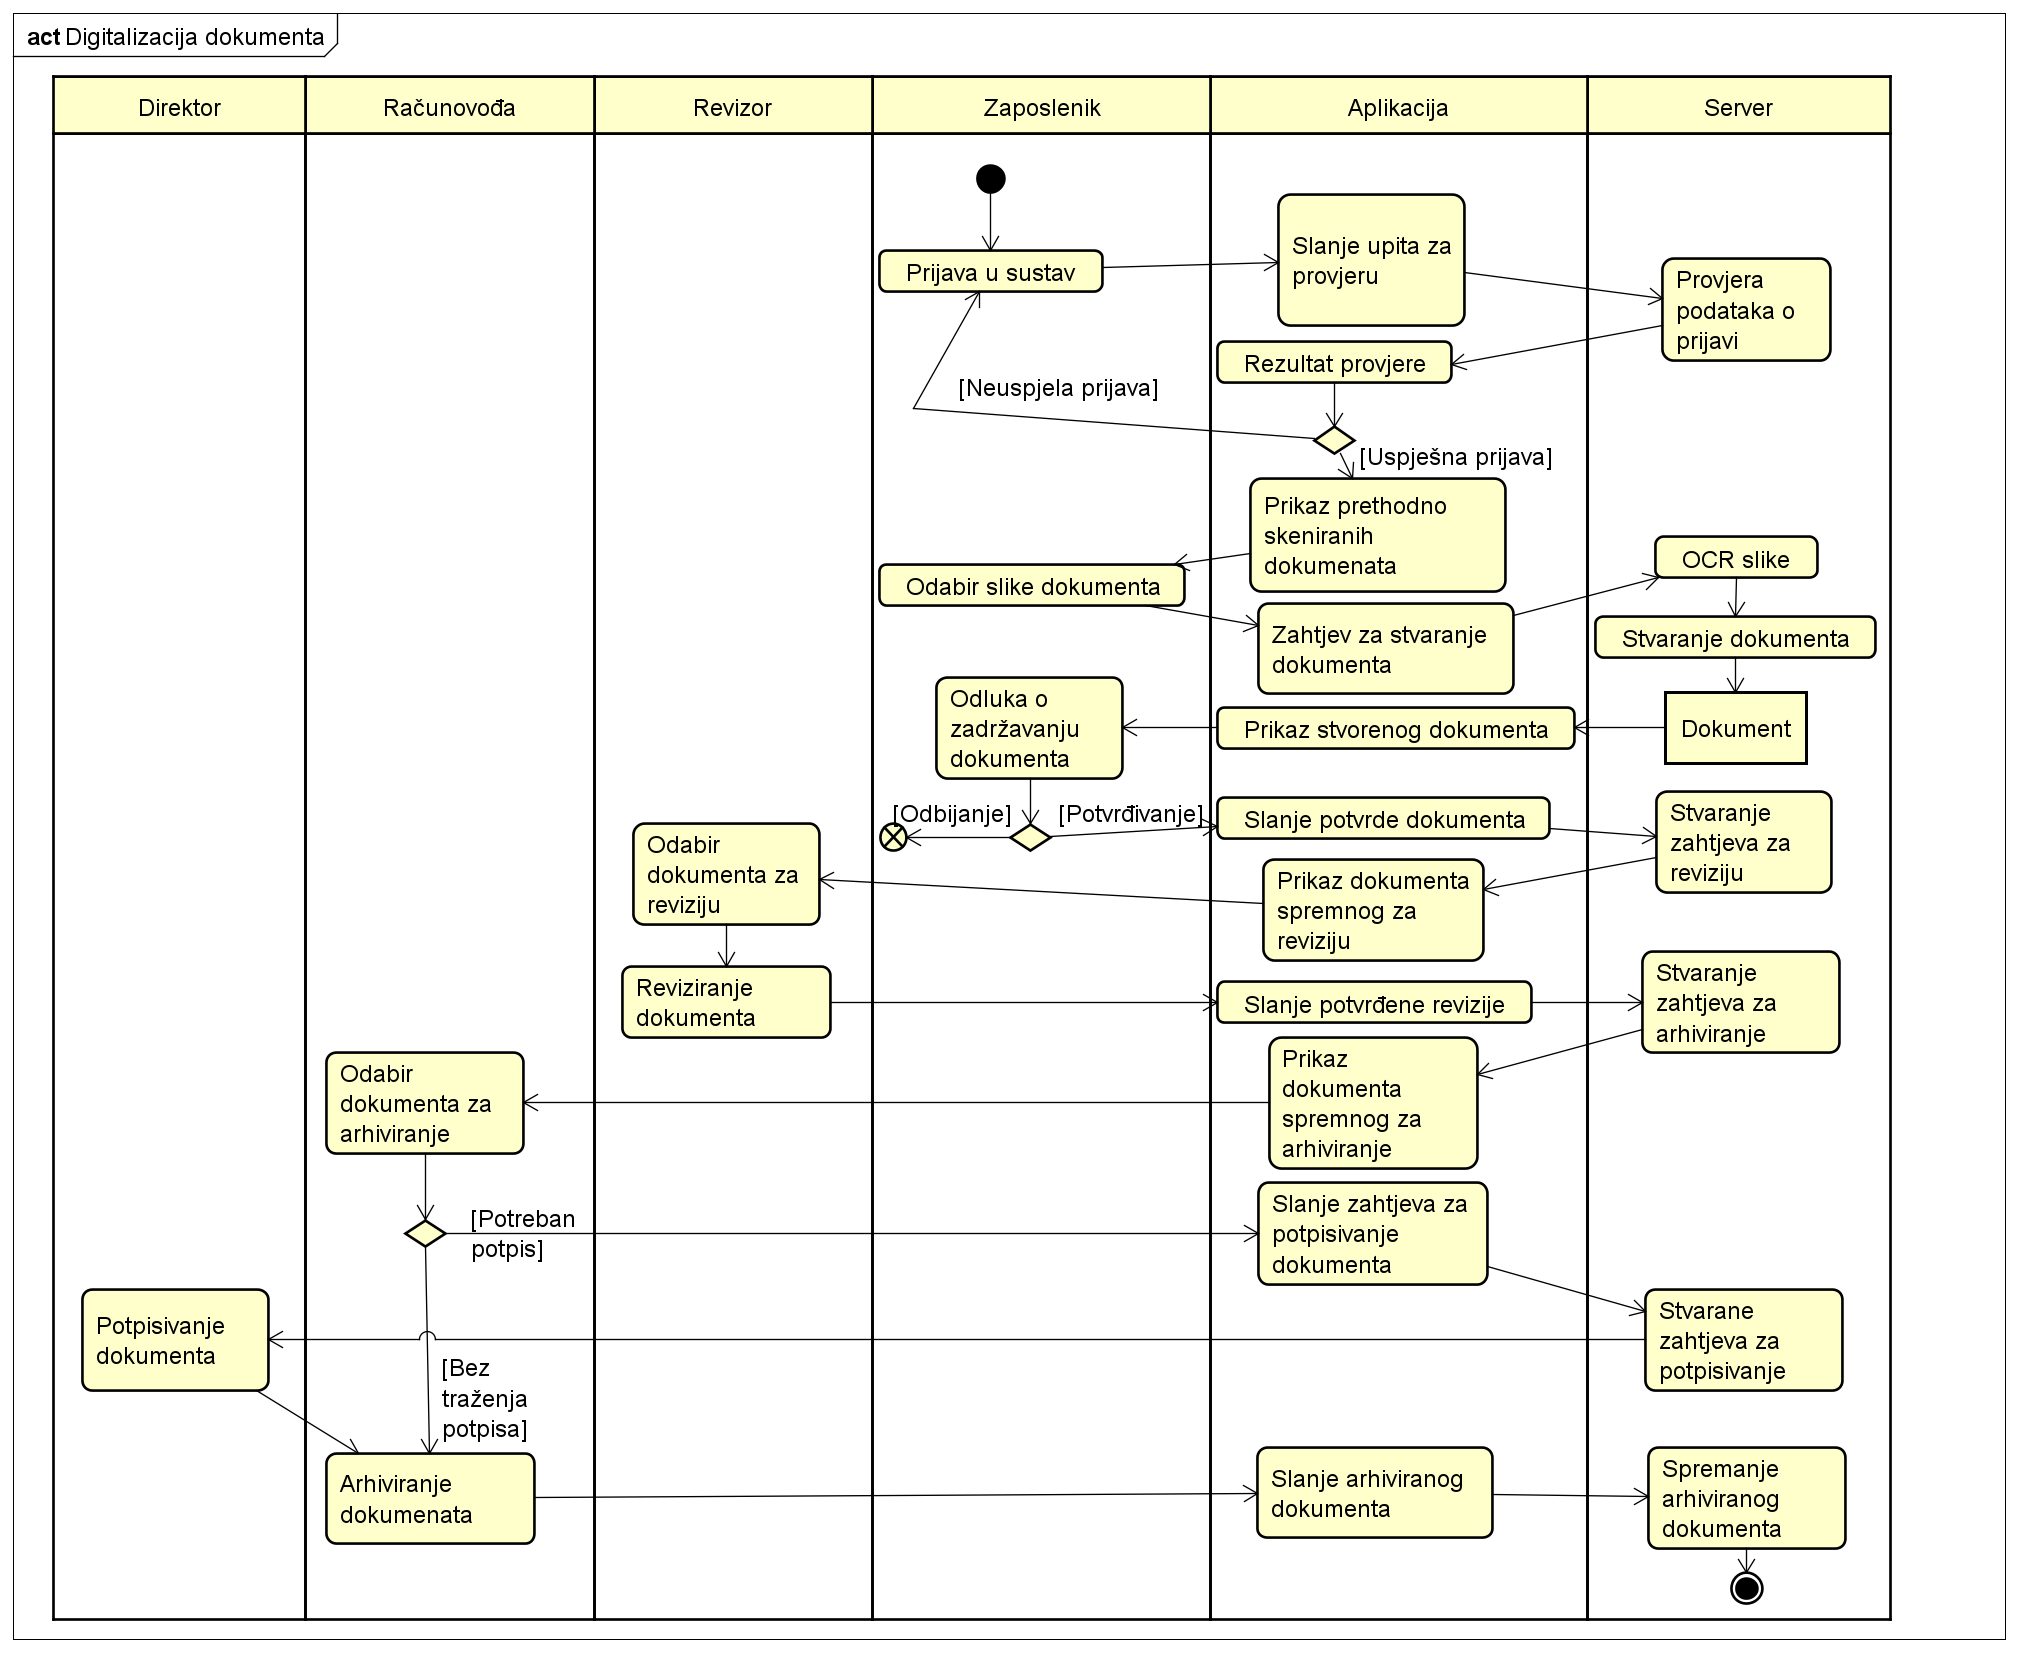
\includegraphics[width=\textwidth]{slike/dijagramAktivnosti.png}
			 	\caption{Dijagram aktivnosti - digitalizacija dokumenta}
			 	\label{fig:dijagramAktivnosti}
			 \end{figure}
			\eject
		\section{Dijagram komponenti}
		
			%\textbf{\textit{dio 2. revizije}}\\
		
			 %\textit{Potrebno je priložiti dijagram komponenti s pripadajućim opisom. Dijagram komponenti treba prikazivati strukturu cijele aplikacije.}
			 
			 {Dijagram komponenti prikazan na slici 4.5 opisuje organizaciju komponenti, internih struktura i komunikaciju različitih dijelova aplikacije. Sustav možemo podijeliti na 2 cjeline: \textbf{Flutter mobilnu aplikaciju} i \textbf{FastAPI backend}. Korisničko sučelje se nalazi unutar \textbf{Flutter mobilne aplikacije}, te sve korisničke interakcije su unutar te mobilne aplikacije. Aplikacija se sastoji od hijerarhije \textit{Flutter widgeta}, koji su zapravo manje cjeline koje grade korisničko sučelje. Interakcijom s korisničkim sučeljem, widget s pomoću \textit{ApiServiceProvidera} koristi \textit{ApiService} te taj servis dohvaća JSON podatke s backend dijela aplikacije. FastAPI backend je REST API i on s pomoću \textit{routera} preusmjerava requestove pripadajućem servisu koji ih dalje preusmjerava pripadajućim \textit{CRUD} klasama. \textit{CRUD} klase zatim preko \textit{Modela} s pomoću \textit{SQLAlchemy}-a dohvaćaju podatke iz baze podataka ili slike s pohrane na oblaku. Ti podaci su pri komunikaciji u obliku \textit{model} objekata ili \textit{schema} pri obrađivanju zahtjeva i odgovoru na njih. Ovisno o JSON podacima koji su se dobili s backenda, frontend prilagođava svoje sučelje.}
			 \begin{figure}[H]
			 	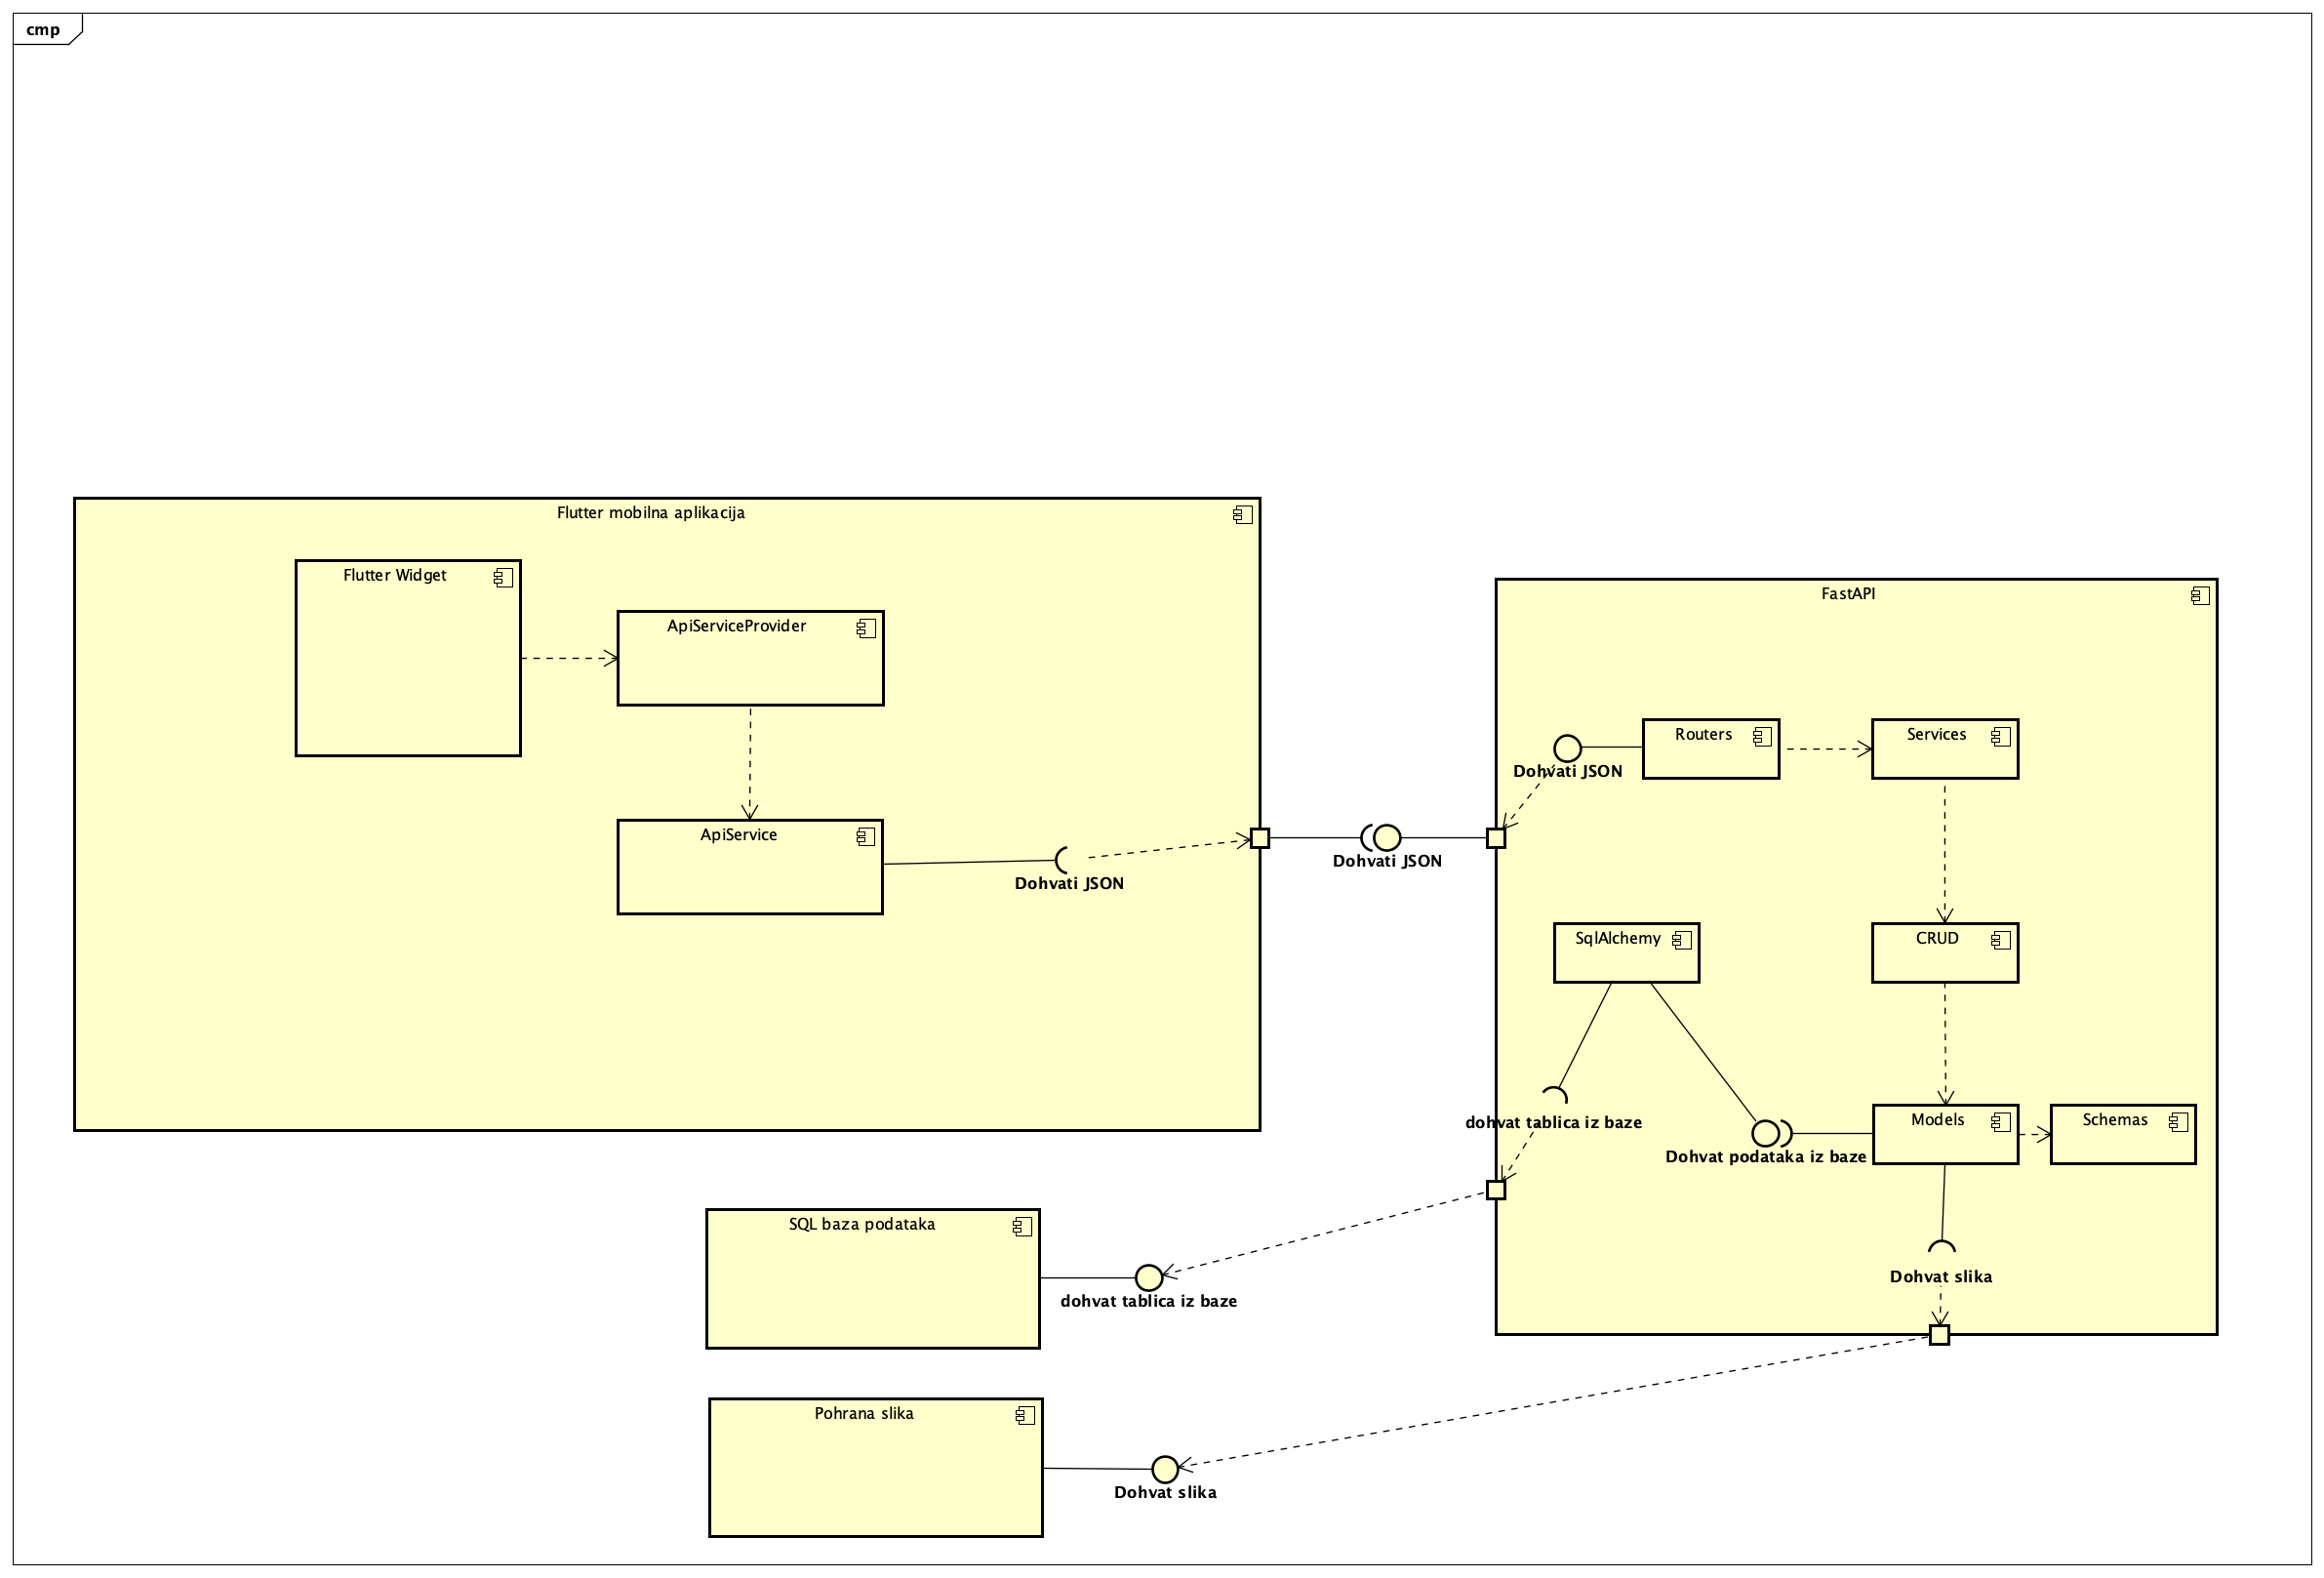
\includegraphics[width=\textwidth]{slike/dijagramKomponenti.png}
			 	\caption{Dijagram komponenti}
			 	\label{fig:dijagramKomponenti}
			 \end{figure}
	\chapter{Implementacija i korisničko sučelje}
		
		
		\section{Korištene tehnologije i alati}
		
			 {Za komunikaciju unutar tima koristili smo \textbf{Whatsapp}\footnote{\url{https://www.whatsapp.com/}} i \textbf{Discord}\footnote{\url{https://discord.com/}}. Za izradu UML dijagrama koristili smo: \textbf{dbdiagram}\footnote{\url{https://dbdiagram.io/}} za dijagram baze podataka, \textbf{Visual Paradigm Online}\footnote{\url{https://online.visual-paradigm.com/}} za dijagram razreda te \textbf{Astah}\footnote{\url{https://astah.net/}} za ostale UML dijagrame. Kao sustav upravljanja verzijama je korišten \textbf{Git}\footnote{\url{https://git-scm.com/}} te su naši repozitoriji bili dostupni na \textbf{Githubu}\footnote{\url{https://github.com/}} udaljenom repozitoriju.
			 	
		 	Kao razvojno okruženje je korišten \textbf{PyCharm}\footnote{\url{https://www.jetbrains.com/pycharm/}} za razvoj API-ja te \textbf{Android Studio}\footnote{\url{https://developer.android.com/studio}} za razvoj mobilne aplikacije. Pycharm je razvojno okruženje za python, napravljeno od JetBrains-a te Android Studio je modificirana inačica drugog JetBrains razvojnog okruženja (IntelliJ, razvojno okruženje za Javu), prilagođena razvoju android mobilnih aplikacija.
		 	
		 	Mobilna aplikacija je napravljena s pomoću \textbf{Flutter}\footnote{\url{https://flutter.dev/}} razvojnog okvira koji koristi \textbf{Dart}\footnote{\url{https://dart.dev/}} programski jezik. Flutter i Dart su projekti razvijeni od strane Googlea. Flutter je razvojni okvir za izradu aplikacija na različitim platformama, vrlo popularan zbog mogućnosti kreiranja aplikacije za više platforma paralelno. Dart je moderni programski jezik koji se primarno koristi za razvoj Flutter aplikacija.
		 	API je kreiran s pomoću \textbf{Pythona}\footnote{\url{https://www.python.org/}} te \textbf{FastAPI}\footnote{\url{https://fastapi.tiangolo.com/}} razvojnog okvira. FastAPI je novije razvojno okruženje bazirano na Flasku, vrlo popularnom python razvojnom okruženju, s mogućnosti paralelnog izvođenja zahtjeva te automatskom dokumentacijom po OpenAPI standardu.
		 	
		 	Aplikacija je puštena u pogon na \textbf{Renderu}\footnote{\url{https://render.com/}}, te je korišten \textbf{Microsoft Azure}\footnote{\url{https://azure.microsoft.com/}}.
	 	 	za spremanje slika, za prepoznavanje teksta na slikama te se tamo nalazi naša baza podataka.
			 }
			 		
			\eject 
		
	
		\section{Ispitivanje programskog rješenja}
			
			\textbf{\textit{dio 2. revizije}}\\
			
			 \textit{U ovom poglavlju je potrebno opisati provedbu ispitivanja implementiranih funkcionalnosti na razini komponenti i na razini cijelog sustava s prikazom odabranih ispitnih slučajeva. Studenti trebaju ispitati temeljnu funkcionalnost i rubne uvjete.}
	
			
			\subsection{Ispitivanje komponenti}
			%\textit{Potrebno je provesti ispitivanje jedinica (engl. unit testing) nad razredima koji implementiraju temeljne funkcionalnosti. Razraditi \textbf{minimalno 6 ispitnih slučajeva} u kojima će se ispitati redovni slučajevi, rubni uvjeti te izazivanje pogreške (engl. exception throwing). Poželjno je stvoriti i ispitni slučaj koji koristi funkcionalnosti koje nisu implementirane. Potrebno je priložiti izvorni kôd svih ispitnih slučajeva te prikaz rezultata izvođenja ispita u razvojnom okruženju (prolaz/pad ispita). }
			
			{Ispitivanje funkcionalnosti sustava provedeno je uz pomoć unit testova. Testirani su service razredi te pripadajući routeri. U nastavku je priloženo nekoliko primjera tih testova te prikaz rezultata testiranja u razvojnom okruženju.\newline}
			
			{Test za razred UserService kojim se testira ispravno kreiranje novog korisnika. Servisu se šalje objekt tipa UserCreate te u slučaju da direktor još ne postoji očekujemo da će povratna vrijednost biti objekt User s podacima o novom korisniku.}
			
\begin{lstlisting}[style=pythonstyle]
	user_create = UserCreate(email="mail@mail.com",	first_name="Test", last_name="Test", username="test", password="test", roles=[RolesEnum.ADMIN],)
	user = User(id=1, email="test@email.com", first_name="Test", last_name="Test", username="test", roles=[],)
	
	def test_register_user():
		mock_user_crud = Mock()
		mock_user_crud.create_user.return_value = user.model_dump()
		mock_user_crud.get_users_by_role.return_value = None
		db = Mock()
		
		user_service = UserService(db)
		
		with patch("app.services.users.UserCRUD", 
					return_value=mock_user_crud):
			result = user_service.register_user(user_create)
		
		mock_user_crud.create_user.assert_called_once_with(user_create)
		mock_user_crud.get_users_by_role.assert_not_called()
		assert result == user.model_dump()
\end{lstlisting}
			
			{Sljedećim testom za documents router testira se reakcija pokušaja dohvaćanja povijesti skeniranih dokumenata za korisnika koji nije ulogiran te se očekuje 'NotAuthenticated' iznimka od servera.}
			
\begin{lstlisting}[style=pythonstyle]
	def test_get_me_not_authenticated():
		response = client.get("/documents/me")
		assert response.status_code == 401
		assert response.json() == {'app_exception': 'NotAuthenticated', 'context': {}}
\end{lstlisting}

			{Test za razred DocumentService koji testira kreiranje dokumenta. Servisu šaljemo sliku i korisničko ime te ako je dokument uspješno kreiran očekujemo da će nam servis vratiti kreirani novi objekt tipa Document sa svim podacima o dokumentu.}
			
\begin{lstlisting}[style=pythonstyle]
	@patch("app.services.documents.detect_document", return_value="R123456 text")
	def test_create_document(detect_document):
		mock_document_crud = Mock()
		mock_document_crud.create_document.return_value = document1
		
		mock_user_service = Mock()
		mock_user_service.get_user.return_value = admin
		
		mock_image_service = Mock()
		mock_image_service.create_image.return_value = imageDB
		db = Mock()
		
		document_service = DocumentService(db)
		
		with patch("app.services.documents.DocumentCRUD", return_value=mock_document_crud), patch("app.services.documents.ImageService", return_value=mock_image_service), patch("app.services.documents.UserService", return_value=mock_user_service):
			result = document_service.create_document(uploaded_image, "username")
		
		detect_document.assert_called_once()
		mock_user_service.get_user.assert_called_once()
		mock_image_service.create_image.assert_called_once()
		
		assert result == document1
\end{lstlisting}

			{Sljedeća dva testa testiraju ažuriranje statusa dokumenta u razredu DocumentService. Prvi provjerava dozvoljeni slučaj iz APPROVED želimo status postaviti na AUDITED, stoga nakon što servisu pošaljemo id dokumenta novi status te eventualne promjene u samom tekstualnom sadržaju očekujemo da će nam vratiti taj dokument s novim statusom. Drugi provjerava slučaj u kojem smo nakon statusa APPROVED odmah skočili na status ARCHIVED. Budući da to nije dozvoljeni slijed statusa očekujemo da će nam servis baciti iznimku "DocumentException.DocumentStatusNotCompatible".}
			
\begin{lstlisting}[style=pythonstyle]
	document2 = Document(id=2, image_id=1, owner=director, document_type=DocumentTypeEnum.INTERNAL, summary="test", document_status=DocumentStatusEnum.APPROVED, scan_time="2021-01-01T00:00:00",)
	document3 = Document(id=2, image_id=1, owner=director, document_type=DocumentTypeEnum.INTERNAL, summary="test", document_status=DocumentStatusEnum.AUDITED, scan_time="2021-01-01T00:00:00",)	

	def test_update_document():
		mock_document_crud = Mock(spec=DocumentCRUD)
		mock_document = Mock(spec=document2, document_status=DocumentStatusEnum.APPROVED)
		mock_document_crud.get_document.return_value = mock_document
		mock_document_crud.update_document.return_value = document3
		db = Mock()
		
		document_service = DocumentService(db)
		
		with patch("app.services.documents.DocumentCRUD", return_value=mock_document_crud):
		result = document_service.update_document(2, DocumentStatusEnum.AUDITED, None)
		
		mock_document_crud.update_document.assert_called_once()
		assert result == document3
	
	def test_update_document_with_invalid_status():
		mock_document_crud = Mock(spec=DocumentCRUD)
		mock_document = Mock(spec=document2, document_status=DocumentStatusEnum.APPROVED)
		mock_document_crud.get_document.return_value = mock_document
		mock_document_crud.update_document.return_value = document3
		db = Mock()
		
		document_service = DocumentService(db)
		
		with patch("app.services.documents.DocumentCRUD", return_value=mock_document_crud):
		with raises(DocumentException.DocumentStatusNotCompatible):
		document_service.update_document(2, DocumentStatusEnum.ARCHIVED, None)
\end{lstlisting}

			{Posljednji testovi testiraju arhiviranje dokumenta u sklopu ArchiveService-a. Dokument se smije arhivirati ako je prethodni status bio PENDING ili SIGNED\textunderscore PENDING. U prvom testu želimo arhivirati dokument čiji status arhiviranja je PENDING te ga želimo postaviti na DONE što je dozvoljeni slijed statusa. Očekuje se uspješni završetak metode archive\textunderscore document koja onda vraća arhivirani dokument s novim statusom DONE.
			U drugom testu želimo isprobati slučaj u kojem pokušavamo dokument iz AWAITING\textunderscore SIGNATURE statusa pretvoriti u DONE što nije dopušteni slijed stanja pa je i očekivano bacanje iznimke "ArchiveException.IllegalArchiveStatus".}
			
\begin{lstlisting}[style=pythonstyle]
	def test_archive_document():
		mock_archive_crud = Mock()
		mock_archive_crud.get_archived_by_document_id.return_value = archive1
		mock_archive_crud.update_archive.return_value = archive1
		
		mock_user_service = Mock(spec=UserService)
		mock_user_service.get_user.return_value = admin
		
		mock_document_service = Mock(spec=DocumentService)
		mock_document_service.update_document.return_value = None
		
		db = Mock()
		
		archive_service = ArchiveService(db)
		
		with patch("app.services.archives.ArchiveCRUD", return_value=mock_archive_crud):
			with patch("app.services.archives.UserService", return_value=mock_user_service):
				with patch("app.services.archives.DocumentService", return_value=mock_document_service):
					result = archive_service.archive_document(1, ArchiveStatus.DONE, "test")
		
		mock_archive_crud.get_archived_by_document_id.assert_called_once_with(1)
		mock_archive_crud.update_archive.assert_called_once()
		assert result == archive1
		
	def test_archive_document_forbidden():
		mock_archive_crud = Mock()
		mock_archive_crud.get_archived_by_document_id.return_value = archive3
		mock_archive_crud.update_archive.return_value = archive1
		
		mock_user_service = Mock(spec=UserService)
		mock_user_service.get_user.return_value = admin
		
		mock_document_service = Mock(spec=DocumentService)
		mock_document_service.update_document.return_value = None
		
		db = Mock()
		
		archive_service = ArchiveService(db)
		
		with patch("app.services.archives.ArchiveCRUD", 	return_value=mock_archive_crud):
			with patch("app.services.archives.UserService", return_value=mock_user_service):
				with patch("app.services.archives.DocumentService", return_value=mock_document_service):
					with raises(ArchiveException.IllegalArchiveStatus):
						archive_service.archive_document(1, ArchiveStatus.DONE, "test")
\end{lstlisting}

			{Svi navedeni ispitni slučajevi prošli su testiranje.}

			\begin{figure}[H]
				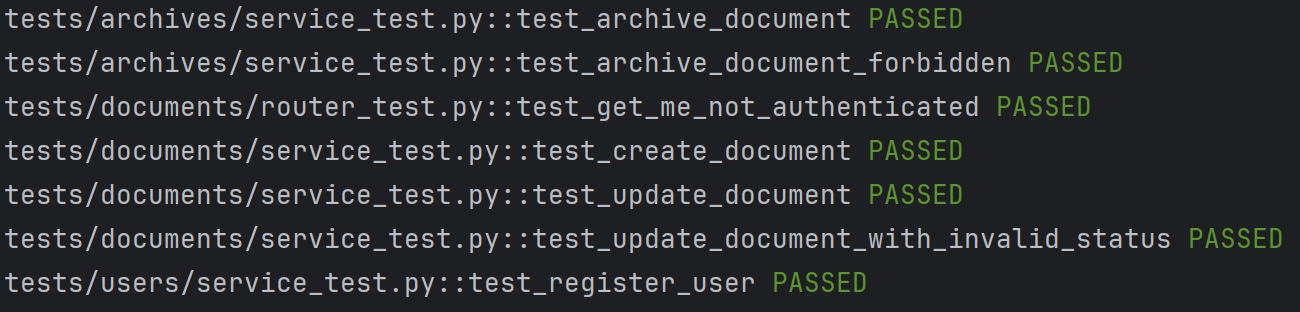
\includegraphics[width=\textwidth]{slike/unitTestovi.png}
				\caption{Prikaz rezultata ispitnih slučajeva u razvojnom okruženju}
				\label{fig:rezultatiUnitTestova}
			\end{figure}		
			
			
			\subsection{Ispitivanje sustava}
			
			 {Razvojni okvir Flutter pruža niz službenih, integriranih alata za izvršavanje više vrsta testova. Ovisno o razini ili dijelu sustava koji se testira dostupni testovi unutar Flutter paketa su Unit, Widget i Integration testovi. Unutar Flutter okvira Integration testovi služe za testiranje čitavog ili pojedinih dijelova sustav, odnosno preuzimaju ulogu integracijskih i sustavnih testova ovisno o implementaciji, a pišu se unutar samog projekta s pomoću jezika Dart, što olakšava održavanje. Integrirani paketi također pružaju mogućnost automatizacije testova, simulacije i praćenja korisničkih unosa, praćenje tijeka izvođenja i mrežnog prometa te lakog pregleda uspješnosti i ispisa provedenih testova. Iz navedenih razloga za testiranje aplikacije korišteni su integrirani alati dostupni unutar paketa flutter\_test i integration\_test. Druga mogućnost bila bi uporaba Appium alata koji se temelji na Selenium strukturi. Dostupni su preko javno održavanih paketa za prilagodbu, no integrirani alati pokazuju se boljim rješenjem za dani slučaj.}
			 
			 {U nastavku su opisani izvedeni testovi sustava. Tijelo svakog testa se sastoji od grupa, a tijelo svake grupe od podtestova. Sve grupe i podtestovi se vrše slijedno, sukladno hijerarhiji definiranoj u implementaciji te predstavljaju korake i potkorake u testiranju. Cilj sljedećih testova je utvrditi ispunjava li potpuno integrirani sustav zadaće u konkretnim slučajevima i prilagođava li se mogućim rubnim slučajevima. Također se želi sagledati mogu li se svi testovi izvršiti slijedno čime se utvrđuje stabilnost sustava. Za svaki testni slučaj opisani su ulazni podaci i početno stanje, koraci testa, očekivani i stvarni rezultat te ocjena rezultata i tijeka izvođenja.}
			 
			 \subsubsection{Test uspješne i neuspješne prijave te odjave}
			 
			 \begin{itemize}
			 	
			 \item{\textbf{Ulazni podaci:}}
			 \begin{itemize}
			 	\item{username1: admin}
			 	\item{password1: admin}
			 	\item{username2: admin}
			 	\item{password2: neadmin}
			 \end{itemize}
			 
			 \item{\textbf{Početno stanje:} Aplikacija u početnom stanju bez prijavljenog korisnika.}
			 
			 \item{\textbf{Koraci testa:} Koraci koji se provode u testu jesu; upisivanje prvih ulaznih podataka u formular za prijavu i pritisak na gumb za prijavu, navigacija na home screen, otvaranje sučelja za navigaciju i pritisak na gumb za odjavu, upisivanje drugih ulaznih podatak u formular za prijavu i pritisak na gumb za prijavu}
			 
			 \item{\textbf{Očekivani rezultat:} Očekuje se navigacija na home screen nakon upisa valjanih podataka za prijavu, pravilno otvaranje sučelja za navigaciju, povratak na login screen te ostanak na istom nakon upisa nevaljanih podataka}
			 
			 \item{\textbf{Stvarni rezultat:} Provedeni koraci se poklapaju s očekivanim, test prolazi}
			 
			 \item{\textbf{Ocjena:} Testirane funkcionalnosti su zadovoljavajuće, rade ispravno, no može se primijetiti nedostatak povratnih informacija pri neuspješnom prijavljivanju zbog neimplementiranih funkcionalnosti}
			 
			\end{itemize}
			
			\subsubsection{Test pregleda korisnika}
			
			\begin{itemize}
				
				\item{\textbf{Ulazni podaci:}}
				\begin{itemize}
					\item{username: owner}
					\item{password: owner}
				\end{itemize}
				
				\item{\textbf{Početno stanje:} Aplikacija u početnom stanju bez prijavljenog korisnika.}
				
				\item{\textbf{Koraci testa:} Koraci koji se provode u testu jesu; upisivanje prvih ulaznih podataka u formular za prijavu i pritisak na gumb za prijavu, navigacija na home screen, otvaranje sučelja za navigaciju i pritisak na gumb za odjavu, upisivanje drugih ulaznih podatak u formular za prijavu i pritisak na gumb za prijavu}
				
				\item{\textbf{Očekivani rezultat:} Očekuje se navigacija na home screen nakon upisa valjanih podataka za prijavu, pravilno otvaranje sučelja za navigaciju, povratak na login screen te ostanak na istom nakon upisa nevaljanih podataka}
				
				\item{\textbf{Stvarni rezultat:} Provedeni koraci se poklapaju s očekivanim, test prolazi}
				
				\item{\textbf{Ocjena:} Testirane funkcionalnosti su zadovoljavajuće, rade ispravno, no može se primijetiti nedostatak povratnih informacija pri neuspješnom prijavljivanju zbog neimplementiranih funkcionalnosti}
				
			\end{itemize}
			
			\subsubsection{Test pregleda dokumenata}
			
			\begin{itemize}
				
				\item{\textbf{Ulazni podaci:}}
				\begin{itemize}
					\item{username: owner}
					\item{password: owner}
				\end{itemize}
				
				\item{\textbf{Početno stanje:} Aplikacija u početnom stanju bez prijavljenog korisnika.}
				
				\item{\textbf{Koraci testa:} Koraci koji se provode u testu jesu; upisivanje prvih ulaznih podataka u formular za prijavu i pritisak na gumb za prijavu, navigacija na home screen, otvaranje sučelja za navigaciju i pritisak na gumb za odjavu, upisivanje drugih ulaznih podatak u formular za prijavu i pritisak na gumb za prijavu}
				
				\item{\textbf{Očekivani rezultat:} Očekuje se navigacija na home screen nakon upisa valjanih podataka za prijavu, pravilno otvaranje sučelja za navigaciju, povratak na login screen te ostanak na istom nakon upisa nevaljanih podataka}
				
				\item{\textbf{Stvarni rezultat:} Provedeni koraci se poklapaju s očekivanim, test prolazi}
				
				\item{\textbf{Ocjena:} Testirane funkcionalnosti su zadovoljavajuće, rade ispravno, no može se primijetiti nedostatak povratnih informacija pri neuspješnom prijavljivanju zbog neimplementiranih funkcionalnosti}
				
			\end{itemize}
			
			\subsubsection{Test revizije dokumenata}
			
			\begin{itemize}
				
				\item{\textbf{Ulazni podaci:}}
				\begin{itemize}
					\item{username: revizor1}
					\item{password: revizor1}
				\end{itemize}
				
				\item{\textbf{Početno stanje:} Aplikacija u početnom stanju bez prijavljenog korisnika.}
				
				\item{\textbf{Koraci testa:} Koraci koji se provode u testu jesu; upisivanje prvih ulaznih podataka u formular za prijavu i pritisak na gumb za prijavu, navigacija na home screen, otvaranje sučelja za navigaciju i pritisak na gumb za odjavu, upisivanje drugih ulaznih podatak u formular za prijavu i pritisak na gumb za prijavu}
				
				\item{\textbf{Očekivani rezultat:} Očekuje se navigacija na home screen nakon upisa valjanih podataka za prijavu, pravilno otvaranje sučelja za navigaciju, povratak na login screen te ostanak na istom nakon upisa nevaljanih podataka}
				
				\item{\textbf{Stvarni rezultat:} Provedeni koraci se poklapaju s očekivanim, test prolazi}
				
				\item{\textbf{Ocjena:} Testirane funkcionalnosti su zadovoljavajuće, rade ispravno, no može se primijetiti nedostatak povratnih informacija pri neuspješnom prijavljivanju zbog neimplementiranih funkcionalnosti}
				
			\end{itemize}
			
			\subsubsection{Test arhiviranja dokumenata}
			
			\begin{itemize}
				
				\item{\textbf{Ulazni podaci:}}
				\begin{itemize}
					\item{username: racunovoda1}
					\item{password: racunovoda1}
				\end{itemize}
				
				\item{\textbf{Početno stanje:} Aplikacija u početnom stanju bez prijavljenog korisnika.}
				
				\item{\textbf{Koraci testa:} Koraci koji se provode u testu jesu; upisivanje prvih ulaznih podataka u formular za prijavu i pritisak na gumb za prijavu, navigacija na home screen, otvaranje sučelja za navigaciju i pritisak na gumb za odjavu, upisivanje drugih ulaznih podatak u formular za prijavu i pritisak na gumb za prijavu}
				
				\item{\textbf{Očekivani rezultat:} Očekuje se navigacija na home screen nakon upisa valjanih podataka za prijavu, pravilno otvaranje sučelja za navigaciju, povratak na login screen te ostanak na istom nakon upisa nevaljanih podataka}
				
				\item{\textbf{Stvarni rezultat:} Provedeni koraci se poklapaju s očekivanim, test prolazi}
				
				\item{\textbf{Ocjena:} Testirane funkcionalnosti su zadovoljavajuće, rade ispravno, no može se primijetiti nedostatak povratnih informacija pri neuspješnom prijavljivanju zbog neimplementiranih funkcionalnosti}
				
			\end{itemize}
			 
			\eject 
		
		
		\section{Dijagram razmještaja}
			
			\textbf{\textit{dio 2. revizije}}
			
			 \textit{Potrebno je umetnuti \textbf{specifikacijski} dijagram razmještaja i opisati ga. Moguće je umjesto specifikacijskog dijagrama razmještaja umetnuti dijagram razmještaja instanci, pod uvjetom da taj dijagram bolje opisuje neki važniji dio sustava.}
			
			\eject 
		
		\section{Upute za puštanje u pogon}
		
			\textbf{\textit{dio 2. revizije}}\\
		
			 \textit{U ovom poglavlju potrebno je dati upute za puštanje u pogon (engl. deployment) ostvarene aplikacije. Na primjer, za web aplikacije, opisati postupak kojim se od izvornog kôda dolazi do potpuno postavljene baze podataka i poslužitelja koji odgovara na upite korisnika. Za mobilnu aplikaciju, postupak kojim se aplikacija izgradi, te postavi na neku od trgovina. Za stolnu (engl. desktop) aplikaciju, postupak kojim se aplikacija instalira na računalo. Ukoliko mobilne i stolne aplikacije komuniciraju s poslužiteljem i/ili bazom podataka, opisati i postupak njihovog postavljanja. Pri izradi uputa preporučuje se \textbf{naglasiti korake instalacije uporabom natuknica} te koristiti što je više moguće \textbf{slike ekrana} (engl. screenshots) kako bi upute bile jasne i jednostavne za slijediti.}
			
			
			 \textit{Dovršenu aplikaciju potrebno je pokrenuti na javno dostupnom poslužitelju. Studentima se preporuča korištenje neke od sljedećih besplatnih usluga: \href{https://aws.amazon.com/}{Amazon AWS}, \href{https://azure.microsoft.com/en-us/}{Microsoft Azure} ili \href{https://www.heroku.com/}{Heroku}. Mobilne aplikacije trebaju biti objavljene na F-Droid, Google Play ili Amazon App trgovini.}
			
			
			\eject 
	\chapter{Zaključak i budući rad}
		
		\textbf{\textit{dio 2. revizije}}\\
		
		 \textit{U ovom poglavlju potrebno je napisati osvrt na vrijeme izrade projektnog zadatka, koji su tehnički izazovi prepoznati, jesu li riješeni ili kako bi mogli biti riješeni, koja su znanja stečena pri izradi projekta, koja bi znanja bila posebno potrebna za brže i kvalitetnije ostvarenje projekta i koje bi bile perspektive za nastavak rada u projektnoj grupi.}
		
		 \textit{Potrebno je točno popisati funkcionalnosti koje nisu implementirane u ostvarenoj aplikaciji.}
		
		\eject 
	\chapter*{Popis literature}
		\addcontentsline{toc}{chapter}{Popis literature}
	 	
 		\textbf{\textit{Kontinuirano osvježavanje}}
	
		\textit{Popisati sve reference i literaturu koja je pomogla pri ostvarivanju projekta.}
		
		
		\begin{enumerate}
			
			
			\item  Programsko inženjerstvo, FER ZEMRIS, \url{http://www.fer.hr/predmet/proinz}
			
			\item  I. Sommerville, "Software engineering", 8th ed, Addison Wesley, 2007.
			
			\item  T.C.Lethbridge, R.Langaniere, "Object-Oriented Software Engineering", 2nd ed. McGraw-Hill, 2005.
			
			\item  I. Marsic, Software engineering book``, Department of Electrical and Computer Engineering, Rutgers University, \url{http://www.ece.rutgers.edu/~marsic/books/SE}
			
			\item  The Unified Modeling Language, \url{https://www.uml-diagrams.org/}
			
			\item  Astah Community, \url{http://astah.net/editions/uml-new}
		\end{enumerate}
		
		 
	
	
	\begingroup
	\renewcommand*\listfigurename{Indeks slika i dijagrama}
	%\renewcommand*\listtablename{Indeks tablica}
	%\let\clearpage\relax
	\listoffigures
	%\vspace{10mm}
	%\listoftables
	\endgroup
	\addcontentsline{toc}{chapter}{Indeks slika i dijagrama}


	
	\eject 
		
	\chapter*{Dodatak: Prikaz aktivnosti grupe}
		\addcontentsline{toc}{chapter}{Dodatak: Prikaz aktivnosti grupe}
		
		\section*{Dnevnik sastajanja}
		
		\begin{packed_enum}
			
			\item  sastanak
			\item[] \begin{packed_item}
				\item Datum: 13. listopad 2023.
				\item Prisustvovali: Tvrtko Puškarić, Luka Bradarić Lisić, Karlo Grgičin, Jura Hostić, Andrea Milanović, Katarina Pešić, Martin Subotić
				\item Teme sastanka:
				\begin{packed_item}
					\item Početni dogovori vezano za odabir teme projekta
					\item Upoznavanje sa kolegama
					\item Pregled predložene teme
					\item Razrada novo-predložene teme
				\end{packed_item}
			\end{packed_item}
			
			\item  sastanak
			\item[] \begin{packed_item}
				\item Datum: 28. listopad 2023.
				\item Prisustvovali: Tvrtko Puškarić, Luka Bradarić Lisić, Karlo Grgičin, Jura Hostić, Andrea Milanović, Katarina Pešić, Martin Subotić
				\item Teme sastanka:
				\begin{packed_item}
					\item Odlučivanje između tema
					\item Razrada odlučenog projekta
					\item Odabir platforme za izradu aplikacije
					\item Raspodijela kolega za zaduženja
					\item Upoznavanje sa LaTex dokumentacijom
				\end{packed_item}
			\end{packed_item}
			
			\item  sastanak
			\item[] \begin{packed_item}
				\item Datum: 5.studenoga 2023.
				\item Prisustvovali: Tvrtko Puškarić, Luka Bradarić Lisić, Karlo Grgičin, Jura Hostić, Andrea Milanović, Katarina Pešić, Martin Subotić
				\item Teme sastanka:
				\begin{packed_item}
					\item Početak slaganja dokumentacije
					\item Upoznavanje kolega zaduženih za mobilnu aplikacijom sa Flutter/Dart razvojnom okolinom
					\item Upoznavanje kolega zaduženih za pozadinski server sa FastAPI/Python razvojnom okolinom
					\item Održana interna radionica korištenja Git platforme
					\item Raspodijela kolega za izradu početnog dijela dokumentacije
				\end{packed_item}
			\end{packed_item}
			
			\item  sastanak
			\item[] \begin{packed_item}
				\item Datum: 8.studenoga 2023.
				\item Prisustvovali: Tvrtko Puškarić, Luka Bradarić Lisić, Karlo Grgičin, Jura Hostić, Andrea Milanović, Katarina Pešić, Martin Subotić
				\item Teme sastanka:
				\begin{packed_item}
					\item Pregled napisane dokumentacije
					\item Početak izrade mobline aplikacije
					\item Početak izrade pozadinskog servera
					\item Pregled modela baze podataka i njezino implementiranje
				\end{packed_item}
			\end{packed_item}
			
			\item  sastanak
			\item[] \begin{packed_item}
				\item Datum: 13.studenoga 2023.
				\item Prisustvovali: Tvrtko Puškarić, Luka Bradarić Lisić, Karlo Grgičin, Jura Hostić, Andrea Milanović, Katarina Pešić, Martin Subotić
				\item Teme sastanka:
				\begin{packed_item}
					\item Finalni pregled napisanje dokumentacije
					\item Testiranje razrađenog dijela mobilne aplikacije i pozadinskog servera
					\item Pregled stanja repozitorija grupe i spajanje u jednu granu
				\end{packed_item}
			\end{packed_item}
			
			%
			
		\end{packed_enum}
		
		\eject
		\section*{Tablica aktivnosti}
		
			\textbf{\textit{Kontinuirano osvježavanje}}\\
			
			 \textit{Napomena: Doprinose u aktivnostima treba navesti u satima po članovima grupe po aktivnosti.}

			\begin{longtblr}[
					label=none,
				]{
					vlines,hlines,
					width = \textwidth,
					colspec={X[7, l]X[1, c]X[1, c]X[1, c]X[1, c]X[1, c]X[1, c]X[1, c]}, 
					vline{1} = {1}{text=\clap{}},
					hline{1} = {1}{text=\clap{}},
					rowhead = 1,
				} 
			
				\SetCell[c=1]{c}{} & \SetCell[c=1]{c}{\rotatebox{90}{\textbf{Tvrtko Puškarić}}} & \SetCell[c=1]{c}{\rotatebox{90}{\textbf{Luka Bradarić Lisić }}} &	\SetCell[c=1]{c}{\rotatebox{90}{\textbf{Karlo Grgičin }}} & \SetCell[c=1]{c}{\rotatebox{90}{\textbf{Jura Hostić }}} &	\SetCell[c=1]{c}{\rotatebox{90}{\textbf{Andrea Milanović }}} & \SetCell[c=1]{c}{\rotatebox{90}{\textbf{Katarina Pešić }}} &	\SetCell[c=1]{c}{\rotatebox{90}{\textbf{Martin Subotić }}} \\  
				Upravljanje projektom 		&  &  &  &  &  &  & \\ 
				Opis projektnog zadatka 	&  &  &  &  &  &  & \\ 
				
				Funkcionalni zahtjevi       &  &  &  &  &  &  &  \\ 
				Opis pojedinih obrazaca 	&  &  &  &  &  &  &  \\ 
				Dijagram obrazaca 			&  &  &  &  &  &  &  \\ 
				Sekvencijski dijagrami 		&  &  &  &  &  &  &  \\ 
				Opis ostalih zahtjeva 		&  &  &  &  &  &  &  \\ 

				Arhitektura i dizajn sustava	 &  &  &  &  &  &  &  \\ 
				Baza podataka				&  &  &  &  &  &  &   \\ 
				Dijagram razreda 			&  &  &  &  &  &  &   \\ 
				Dijagram stanja				&  &  &  &  &  &  &  \\ 
				Dijagram aktivnosti 		&  &  &  &  &  &  &  \\ 
				Dijagram komponenti			&  &  &  &  &  &  &  \\ 
				Korištene tehnologije i alati 		&  &  &  &  &  &  &  \\ 
				Ispitivanje programskog rješenja 	&  &  &  &  &  &  &  \\ 
				Dijagram razmještaja			&  &  &  &  &  &  &  \\ 
				Upute za puštanje u pogon 		&  &  &  &  &  &  &  \\  
				Dnevnik sastajanja 			&  &  &  &  &  &  &  \\ 
				Zaključak i budući rad 		&  &  &  &  &  &  &  \\  
				Popis literature 			&  &  &  &  &  &  &  \\  
				&  &  &  &  &  &  &  \\ \hline 
				\textit{Dodatne stavke kako ste podijelili izradu aplikacije} 			&  &  &  &  &  &  &  \\ 
				\textit{npr. izrada početne stranice} 				&  &  &  &  &  &  &  \\  
				\textit{izrada baze podataka} 		 			&  &  &  &  &  &  & \\  
				\textit{spajanje s bazom podataka} 							&  &  &  &  &  &  &  \\ 
				\textit{back end} 							&  &  &  &  &  &  &  \\  
				 							&  &  &  &  &  &  &\\ 
			\end{longtblr}
					
					
		\eject
		\section*{Dijagrami pregleda promjena}
		
		\textbf{\textit{dio 2. revizije}}\\
		
		\textit{Prenijeti dijagram pregleda promjena nad datotekama projekta. Potrebno je na kraju projekta generirane grafove s gitlaba prenijeti u ovo poglavlje dokumentacije. Dijagrami za vlastiti projekt se mogu preuzeti s gitlab.com stranice, u izborniku Repository, pritiskom na stavku Contributors.}
		
	


\end{document} %naredbe i tekst nakon ove naredbe ne ulaze u izgrađen dokument 


